\RequirePackage{fix-cm}
\documentclass{cta-author}

\newtheorem{theorem}{Theorem}{}
\newtheorem{corollary}{Corollary}{}
\newtheorem{remark}{Remark}{}
\newtheorem{definition}{Definition}{}
\newtheorem{lemma}{Lemma}{}
\newtheorem{acknowledgements}{Acknowledgements}{}





%\usepackage{lipsum}

\usepackage{graphicx}
\usepackage{subfig}
\usepackage{tabularx}
\usepackage{array,graphicx}
\usepackage{float}

%\usepackage{cite}
\usepackage{amssymb}
\usepackage{amsmath}
\usepackage{amsfonts}
\usepackage{amscd}
\usepackage{enumerate}
\usepackage{url}
\usepackage{algorithm, algorithmic}
%\usepackage[a4paper,left=2.5cm,right=2cm,top=1.8cm,bottom=1.8cm]{geometry}
\usepackage{upquote}
\usepackage{multicol, multirow}

%\usepackage{slashbox}  % create diagonal line in tables

%\usepackage{hyperref}
%\usepackage[nameinlink]{cleveref}
%\usepackage{tikz}
%\usepackage{mdframed}
%\usepackage{textcomp}


\renewcommand{\algorithmicrequire}{\normalsize \textbf{Input:}}
\renewcommand{\algorithmicensure}{\normalsize \textbf{Output:}}
\renewcommand{\algorithmicwhile}{\normalsize \textbf{while}}

\renewcommand\UrlFont{\color{blue}\rmfamily}
%def
\def\N{\mathbb{N}}
\def\Z{\mathbb{Z}}
\def\Q{\mathbb{Q}}
\def\R{\mathbb{R}}
\def\C{\mathbb{C}}
\def\F{\mathbb{F}}


\usepackage{color}
\usepackage{listings} 
\usepackage{xspace}  % to allow for text macros that don't eat space 
\usepackage[misc,geometry]{ifsym}


\lstdefinelanguage{Sage}[]{Python}
{morekeywords={True,False,sage,singular},
	sensitive=true}
\lstset{frame=none,
	showtabs=False,
	showspaces=False,
	showstringspaces=False,
	commentstyle={\ttfamily\color{dredcolor}},
	keywordstyle={\ttfamily\color{dbluecolor}\bfseries},
	stringstyle ={\ttfamily\color{dgraycolor}\bfseries},
	language = Sage,
	basicstyle={\small \ttfamily},
	aboveskip=.3em,
	belowskip=.1em
}
\definecolor{dblackcolor}{rgb}{0.0,0.0,0.0}
\definecolor{dbluecolor}{rgb}{.01,.02,0.7}
\definecolor{dredcolor}{rgb}{0.8,0,0}
\definecolor{dgraycolor}{rgb}{0.30,0.3,0.30}
\newcommand{\dblue}{\color{dbluecolor}\bf}
\newcommand{\dred}{\color{dredcolor}\bf}
\newcommand{\dblack}{\color{dblackcolor}\bf}

\renewcommand{\emph}[1]{{\dblack{#1}}}

\newcommand{\Sage}{{\color{dbluecolor}\sf Sage}\xspace}




\begin{document}
	
	\supertitle{Submission Template for IET Research Journal Papers}
	
	\title{Impact of Modulus Switching Technique on Some Attacks against Learning Problems}
	
	\author{\au{Huy Quoc Le$^{1\corr}$}, \au{Pradeep Kumar Mishra $^{1}$}, \au{Satoshi Nakamura $^{1}$}, \au{Koha Kinjo $^{2}$}, \au{Dung Hoang Duong$^{3}$}, \au{Masaya Yasuda$^{4,5}$}}
	
	\address{\add{1}{Graduate School of Mathematics, Kyushu University, 744 Motooka, Nishi-ku, Fukuoka-shi, Fukuoka-ken, 819-0395, Japan}
			\add{2}{NTT Secure Platform Laboratories, Japan}
		\add{3}{School of Computing and Information Technology, University of Wollongong, Northfields Avenue, Wollongong NSW 2522, Australia}
		\add{4}{Institute of Mathematics for Industry, Kyushu University,
			744 Motooka, Nishi-ku, Fukuoka-shi, Fukuoka-ken, 819-0395, Japan}
		\add{5}{JST, CREST, 4-1-8 Honcho, Kawaguchi, Saitama, 332-0012, Japan.}
		\email{huyle84@gmail.com}}
	
 
\begin{abstract}
	 \looseness=-1 The modulus switching technique has been used in some cryptographic applications as well as in cryptanalysis.  For cryptanalysis against the Learning with Errors (LWE) problem and the Learning with Rounding (LWR) problem, it seems that one does not know whether the technique is really useful or not. This work supplies a complete view of the impact of this technique on the decoding attack, the dual attack and the primal attack against both LWE and LWR. For each attack, we give the optimal formula for the switching modulus. The formulas get involved the number of LWE/LWR samples which differs from the known formula in the literature. We also attain the corresponding sufficient conditions saying when we should utilize the technique. Surprisingly, restricted to the LWE/LWR problem that the secret vector is much shorter than the error vector, we also show that performing the modulus switching before using the so-called \textit{rescaling} technique in the dual attack and the primal attack make these attacks worse than only exploiting the rescaling technique as reported by Bai and Galbraith for their attack at ACISP 2014. As an application, we theoretically assess the influence of the modulus switching on the LWE/LWR-based second round NIST PQC submissions.
	
	
\end{abstract}

\maketitle

%===============
\section{Introduction}
%===============


Quantum computers that are machines exploiting quantum-mechanical phenomena are supposed to be more powerful than conventional computers. If such a machine is built, despite that the machine will be very useful in many beneficially real applications thanks to its power, it can also be used in compromising the digital world and hence the real world. In fact, if a large-scale quantum computer becomes real, many of the public-key cryptosystems that based on classical hard problems  (e.g., the Integer Factorisation Problem or the Discrete Logarithm Problem or the Elliptic Curve Problem) currently in use could be broken due to the quantum computers' capacity in efficiently solving mathematical problems that are difficult or intractable for classical computers \cite{Sho97}. Under the threat of quantum computers, lattice-based cryptography, among others \cite{Ber09}, has become a leading candidate for being against the power of these quantum machines. 


Among many lattice problems, LWE has been becoming a very important problem in lattice-based cryptography since its introduction in the seminal work of Regev \cite{Reg09} in 2005. The problem uses a noise sampled from some distribution (typically, Gaussian distribution) to hide the secret key. So far, the problem has been well-studied and has been playing a crucial role as an underlying hard problem utilized to built various public-key cryptosystems \cite{Reg09, Pei09, GPV08}. A disadvantage of the original LWE problem is that the noise is drawn from the discrete Gaussian distribution which is costly to implement in practice. In 2010, a de-randomization variant of LWE using a rounding operation to conceal the secret key instead of a discrete Gaussian noise, the LWR problem, was introduced by Banerjee, Peikert and Rosen \cite{BPR12}. The LWR problem has also several applications in lattice-based cryptography such as pseudorandom functions \cite{BPR12}, lossy trapdoor functions, reusable extractors \cite{AKPW13}, key homomorphic pseudorandom functions \cite{BLMR13}, etc.  


\begin{table}[pt]
	\caption{\textbf{The Second-Round NIST PQC Submissions based on LWE and\\ LWR problems}} 
	\centering
	\small\addtolength{\tabcolsep}{0pt}
	
	\begin{tabular}{ c | c  }
		\hline
		
		\textbf{Cryptosystems}&\textbf{LWE/LWR variants}\\
		\hline
		\hline
		CRYSTALS-Kyber&Module-LWE (MLWE)\\
		FrodoKEM& LWE\\
		LAC&Ring-LWE (RLWE)\\
		NewHope&RLWE\\
		
		Round5 &General LWR \\
		SABER&LWR\\
		ThreeBears&ILWE (Integer version of MLWE) \\
		CRYSTALS-Dilithium&RLWE\\
		qTESLA&RLWE\\
		\hline
	\end{tabular}
	\label{table:21}
\end{table}

In order to prepare for the upcoming post-quantum era, National Institute of Standards and Technology (NIST) processed a competition called \textit{NIST Post-Quantum Cryptography (NIST PQC) Standardization} in November 2017. Among 82 candidate packages in total were submitted to NIST at the beginning of the process, 69 submissions were accepted as First-Round Candidates on December 20, 2017. After that from these submissions, 26 packages were chosen to be the \textit{Second-Round NIST PQC Candidates} (we also refer them as \textit{the second round NIST PQC submissions}) of the competition as announced on January 30, 2019, by the NIST organiser \cite{AAA+19}.  It is noteworthy to know that there are up to 9 Second-Round NIST PQC Candidates that are based on LWE/LWR and their variants (see also Table \ref{table:21} for a summary), whereas the remaining candidates (17 submissions) are NTRU-based, multivariate-based, code-based, hash-based ones, and so forth. Remark that the security, cost and performance, and algorithm and implementation characteristics are criteria that NIST considered in selecting the second round candidates \cite[Subsection 2.3]{AAA+19}. Same as other lattice problems, LWE/LWR variants enjoy very strong security proofs based on worst-case hardness, relatively efficient implementations, as well as great simplicity (cf. \cite{MR09}). These characteristics make LWE/LWE-based candidates important and leading ones for the NIST's consideration.






For more details in the security aspect, the hardness of LWE has been well studied in the literature \cite{Reg09, APS15, BLP+13}. Regev \cite{Reg09} showed that the LWE problem is as hard to solve as several worst-case lattice problems. Also, for LWR, there are some analyses of its hardness based on reducing LWR to LWE under certain constraints on parameters such as \cite{BPR12, AKPW13, BGM+15, AA16}. And, until now, the only known approach in attacking LWR is to transform an LWR instance to an LWE instance. Most of the strategies for breaking LWR are able to be adapted from attacks against an LWE modulo $q$ instance  \cite{BBGM+19, DTV15} such as the dual attack, the decoding attack, the primal attack, algebraic attacks \cite{AG11} and so on (cf. \cite{APS15} for more details). 

In this work, we just focus on the decoding attack, the dual attack and the primal attack. While the first attack was mentioned in our preliminary work \cite{LMDY18}, the second and the third are attacks often mentioned in security analyses of lattice-based NIST PQC submissions. Compared to the decoding attack, the dual attack and the primal attack are much better, especially in the case that the secret (and the noise, the error) is sampled from (even sparse) small sets and that not many numbers of samples are given. For example, the secret key of Round5, a second round NIST PQC candidate, is sampled according to a fixed Hamming weight distribution of support $\{-1, 0, 1\}$, named $\mathcal{H}_{n,k}(h)$, from which each drawn vector of length $n\cdot k$ has exactly $h$ non-zero components \cite{BBGM+19}.  


The modulus switching technique was used for the first time aiming to speed up the homomorphic encryption operations \cite{BV11a}. Then the technique was also used to evaluate the classical hardness of LWE problem \cite{BLP+13}. Recently, the technique was modified to combine with the Blum-Kalai-Wasserman (BKW) algorithm on LWE \cite{AFFP14}. The technique allows to transform an LWE modulo $q$ instance to an LWE modulo $q'$ instance  with $q'$ (called \textit{the switching modulus}) is typically chosen as
\begin{equation}\label{keye}
q' \approx \frac{\sigma_s}{\sigma}\cdot \sqrt{\frac{n}{12}}\cdot q,
\end{equation} 
where $n$ is the length of the secret and $\sigma_{s}$,  $\sigma$ are standard deviations of the secret and the error of the original LWE modulo $q$ instance, respectively (cf. \cite[Lemma 2]{APS15}).  Remark that, Eq. \eqref{keye} does not involve the number of LWE samples $m$. It is noteworthy to know that the number of LWE samples plays an important role in the success of attacks against the LWE problem. The authors of \cite{BBGS18} analyzed the hardness of LWE instances given a restricted number of samples. Since then, they extended the LWE-Estimator of \cite{APS15} which is a software tool used to estimate the hardness of concrete LWE instances and to choose parameters for lattice-based primitives. Furthermore, they also showed the impact of restricting the number of available samples. 

Obviously, Eq. \eqref{keye} just supplies us a commonly used switching modulus $q'$ not aiming to strengthen the power of known attacks.  Also, note that the effect of the modulus switching technique on attacks against the LWE/LWR problems as well as on other techniques, e.g., the so-called rescaling technique, has not been studied carefully so far. The present work is to try to close the gap we have mentioned. 



\begin{table*}[t]
	\caption{\textbf{Choose the optimal switching modulus  $q'$ for some typical attacks against LWE and LWR problems} } 
	\centering
	\small\addtolength{\tabcolsep}{0pt}
	\begin{tabular}{ c || c | c|  c  }
		\hline
		\multirow{2}{*}{\textbf{Attacks}}&\multirow{2}{*}{\textbf{Literature} \cite{APS15}} & \multicolumn{2}{c}{\textbf{Our work}}   \\
	
		&& \textbf{Optimal modulus} & \textbf{Notations}  \\
		\hline
		\hline
		\multirow{2}{*}{Decoding }&\multirow{6}{*}{
			$q' \approx \sqrt{\frac{n\sigma_s^2}{12\sigma^2}}\cdot q $
		}&$q'\approx \sqrt{\frac{(m-n)N}{nM}}$ &$N=n\sigma_s^2$\\
		& & & \\
	
		
		\multirow{2}{*}{Dual}& &$q' \approx \sqrt{\frac{mN}{nM}}$&LWE: $M:=M_{lwe}=\frac{12\sigma_{lwe}^2}{q^2}$ \\ %$\sigma_{lwe}=\frac{\alpha q}{\sqrt{2 \pi}}$\\
			& & & \\
		& $\approx \sqrt{N/M}$& &\\

		\multirow{2}{*}{Primal}  & &\multirow{2}{*}{$q' \approx \sqrt{\frac{(m+12)N}{(n+1)M}}$}&LWR: $M:=M_{lwr}=\frac{q^2+2q}{p^2q^2} \approx \frac{12\sigma_{lwr}^2}{q^2},$\\
		&&& $\sigma_{lwr}=\sqrt{\frac{q^2+2pq}{12p^2}}$\\
		\hline 
	\end{tabular} \label{tab2}
\end{table*}


\paragraph{Our contribution}
 This paper is the extended version of our CANS 2018 paper \cite{LMDY18}.
In general, the present work extends our approach in \cite{LMDY18} to the dual attack and the primal attack for not only LWR but also LWE. 
We processed a complete consideration of the impact of the modulus switching technique being used to solve both LWE and LWR on these typical attacks. More specifically,

	 (i) We set up a common framework for both problems.  To do that, we scrutinized in details transforming from an LWR instance to a corresponding LWE instance as well as the behavior of the induced LWR error. Furthermore, the successful range in which a search LWR instance can be solved by the decoding attack associated with Babai's Nearest Plane algorithm was also determined. Based on the successful range, we take LWR instances that are consistent with our experiments. This is the completed work of \cite{LMDY18}.


	(ii) We obtained the optimal value for the switching modulus with respect to each attack (see Table \ref{tab2} for a summary) accompanied with the sufficient condition for exploiting the modulus switching technique in attacking the LWE/LWR problems. Our optimal formulas for the switching modulus get involved the number of LWE/LWR samples which is different from Eq. \eqref{keye} (see Table \ref{tab3} for a summary and see  also Table \ref{table:7} for a comparison between the values of the switching moduli according to each attack summarized in Table \ref{tab2} and the values of $q'$ according to Eq. \eqref{keye} with some specific parameters). 	


	(iii) We compared the efficacy of the modulus switching and that of the so-called rescaling technique which is mentioned in attacks against LWE/LWR in the case that the secret is much smaller than the error (e.g., the secret is a binary or trinary vector) (see Table \ref{tab4} for a summary).


	(iv) We also assessed the effect of the modulus switching technique on the rescaling technique. Our computation theoretically confirms again the result by Bai and Galbraith at ACISP 2014 \cite{BG14} that their attack which exploits the rescaling technique is weakened by applying the modulus switching. 


	(v) Finally, based on our theoretical results, we also evaluated how the LWE/LWR-based NIST PQC submissions are impacted by the modulus switching.


To the best of our knowledge, this work is the first attempt to evaluate carefully the modulus switching's influence on attacks breaking the LWE/LWR problems. We expect that our work will not only provide with a different perspective in exploiting the modulus switching technique to attack LWR/LWE but also gets more attention in other application scenarios.

\paragraph{Organisation}  Section \ref{pre} gives some background knowledge necessary to our work later on. In Section \ref{reduce}, we first remind the typical way we transform an LWR instance into an LWE instance, then determine the distribution of the induced LWR error. We also estimate the successful range for the decoding attack against LWR in this section.  We will review the modulus switching technique applied to LWE and LWR in Section \ref{sec5}. Choosing the optimal switching modulus for the decoding attack, the dual attack and the primal attack will be conducted in Section \ref{sec4}. In Section \ref{modvsre}, we compare the modulus switching with the so-called rescaling technique when applied separately to attacks. A valuation on the impact of the modulus switching to the efficacy of the rescaling technique will be done in Section \ref{impact}. Section \ref{sec6} presents some experimental results relating to using the modulus switching technique in solving the LWR problem. Section \ref{sec8} is devoted to summarize the second round NIST PQC candidates which rely their security on the hardness of the LWE/LWR variants and evaluate theoretically the impact of the modulus switching on them. Section \ref{conclu} is to conclude our work. 




\begin{table*}[t]
	\small\addtolength{\tabcolsep}{20pt}
	\caption{\textbf{The sufficient condition for that the modulus switching technique is better than the rescaling technique}} 
	\centering
	\small
	\begin{tabular}{c c  }
		\hline
		\textbf{Attacks}& \textbf{Sufficient condition}\\
		\hline\hline
		
		\multirow{2}{*}{Dual}&\multirow{2}{*}{$ \left(\frac{12\sigma^2}{\sigma_s^2}\right)^{n} \geq\frac{(m+n)^{m+n}}{m^{m}}\cdot \frac{\sigma^{2n}}{\sigma_s^{2(m+n)}}$}\\
		&\\
		
		\hline
		\multirow{2}{*}{Primal}  &\multirow{2}{*}{$ \left(\frac{12(N+m\sigma^2)}{m+n+1}\right)^{m+n+1} \geq \left( \frac{(m+12)N}{n+1}\right)^{n+1} \cdot \left( q^{2} M \right)^{m} \cdot \frac{\sigma_s^{2m}}{\sigma^{2m}} $}\\
		&\\
		\hline
	\end{tabular}\label{tab4}
\end{table*}


%==============================
\section{Preliminaries} \label{pre}
%==============================



\subsection{Notations} In this work, we represent (column) vectors in lower bold letters, e.g., vector $\mathbf{a}$, matrices in upper bold letters, e.g., matrix $\mathbf{A}$. We write $\mathbf{v}^t$ (resp. $\mathbf{A}^t$) as the transpose of the vector $\mathbf{v}$ (resp. the matrix $\mathbf{A}$). The norm of a vector $\mathbf{v}$ is the standard Euclidean norm  computed as $\Vert \mathbf{v}\Vert=\sqrt{\langle \mathbf{v}, \mathbf{v}\rangle}$. 



If $S=\{a_1, \cdots ,a_m\}$ with $a_i\in \mathbb{R}$ then $k\cdot S=\{k\cdot  a_1,\cdots,k\cdot  a_m\}$ for any $k\in \mathbb{R}$. The logarithm of base 2 of a positive real number $x$ will be written as $\log (x)$. We use $\mathcal{U}(S)$ to indicate the uniform distribution over the set $S$. The rounding operation $\lfloor a \rceil$ outputs the integer closest to $a$ and in the case of a tie, it outputs the integer next to $a$. For any positive integer $q$, we denote by $\mathbb{Z}_q=\{0,1, \cdots, q-1\}$ the set of integers modulo $q$. By ``$a:=b$'' we mean defining the new variable $a$ by assigning its value to be $b$ 

We write $x \leftarrow \chi$ to say that the random variable $x$ follows the probability distribution $\chi$ or $x$ is sampled from the distribution $\chi$. Let $\mathbf{v}$ be a vector, $\mathbf{A}$ be a matrix and $f$ be a polynomial. Notations like $\mathbf{v} \leftarrow \chi^n$, $\mathbf{A} \leftarrow \chi^{m \times n}$, $f \leftarrow \chi^n$, etc., say that $\mathbf{v}$, $\mathbf{A}$ and $f$  are sampled element-wise or coefficient-wise according to the distribution $\chi$. For a real number $k$, the notation $y \leftarrow k \cdot \chi$ means that $y=k \cdot x$ for some $x$ that follows the probability distribution $\chi$. 

%=======================
\subsection{Lattices}
%=======================

%Let $\mathbf{a}_1,\cdots,\mathbf{a}_{m}$ be $m$ linearly independent vectors in $\mathbb{Z}^n$. 
The lattice $\mathcal{L}=\mathcal{L}(\mathbf{A})$ generated by the column matrix $\mathbf{A}=[\mathbf{a}_1,\cdots,\mathbf{a}_{m} ] \in \mathbb{R}^{n \times m}$ of $m$ linearly independent vectors is defined to be the set of all linear integral combinations of $\mathbf{a}_{i}$'s, i.e., 
$\mathcal{L}(\mathbf{A})=\left\{ \mathbf{A}.\mathbf{x}: \mathbf{x} \in \mathbb{Z}^{m}\right\}=\left\{ \sum_{i=1}^{m} x_i\mathbf{a}_i: x_i \in \mathbb{Z}\right\}.  $
We call the matrix $\mathbf{A}$ \textit{a basis} of $\mathcal{L}$ and call each $\mathbf{a}_i$ \textit{a basis vector}. The \textit{rank} of the lattice is the number of basis vector (i.e., $m$). The \textit{dimension} of the lattice is the number of entries in each basis vector (i.e., $n$). If $m=n$, the lattice is called to be \textit{full-rank}. Notice that, every lattice has infinitely many bases up to a unimodular matrix of determinant $\pm1$. Hence, if $\mathbf{A}$ and $\mathbf{B}$ are two different bases of the lattice $\mathcal{L}$, then $\det (\mathbf{A}^t \mathbf{A})=\det (\mathbf{B}^t \mathbf{B})$. We call $\det(\mathcal{L}(\mathbf{A})):=\sqrt{\det (\mathbf{A}^t \mathbf{A})}$ the \textit{determinant} (or \textit{volume}) of the lattice $\mathcal{L(\mathbf{A})}.$ 

\textit{The Gram-Schmidt} matrix $\mathbf{A}^{*}=[\mathbf{a}^{*}_1,\cdots,\mathbf{a}^{*}_{m} ]$ for a basis $\mathbf{A}=[\mathbf{a}_1,\cdots,\mathbf{a}_{m} ]$ is defined by setting
$\mathbf{a}^{*}_1=\mathbf{a}_1\text{ and } \mathbf{a}^{*}_{i}=\mathbf{a}_{i}-\sum_{j=1}^{i-1} \mu_{i,j}\cdot \mathbf{a}^{*}_j,$ where $\mu_{i, j}=\langle \mathbf{a}_{i}, \mathbf{a}^{*}_j \rangle/\Vert\mathbf{a}^{*}_j\Vert^2,$ for $i=2,\cdots,m.$  We can prove that $\det(\mathcal{L}{(\mathbf{A})})=\prod_{i=1}^{m}\Vert \mathbf{a}_i^* \Vert.$
The \textit{fundamental parallelepiped} associated with a basis $\mathbf{A}=[\mathbf{a}_1,\cdots,\mathbf{a}_{m}]$ is $\mathcal{P}_{1/2}(\mathbf{A})=\left\{ \sum_{i=1}^{m} x_i\mathbf{a}_i: x_i \in \left[-\frac{1}{2},\frac{1}{2} \right)\right\}. $ We define the fundamental parallelepiped $\mathcal{P}_{1/2}(\mathbf{A}^{*})$ for the Gram-Schmidt matrix $\mathbf{A}^{*}$ in the same way. 

There always exist non-zero vectors having the smallest norm and non-zero vectors having the second smallest norm in a lattice $\mathcal{L}$. We call these norms \textit{the first minimum} $\lambda_1(\mathcal{L}
$) and \textit{the second minimum} $\lambda_2(\mathcal{L})
$, respectively. 

Let $\mathcal{L}$ be a lattice of rank $m$ and $S$ be a measurable subset of the  corresponding space $\mathbb{R}^m$, \textit{Gaussian Heuristic} says that  
$\#S \cap \mathcal{L} \approx \text{vol}(S)/\text{det} (\mathcal{L}).$
Consequently, we have the following estimation for the length of the shortest non-zero vectors of $\mathcal{L}$:
\begin{equation*} \label{eqq1}
\lambda_1(\mathcal{L}) \approx \sqrt{\frac{m}{2\pi \mathfrak{e}}}\det(\mathcal{L})^{1/m},
\end{equation*}
where $\mathfrak{e}$ is the mathematical constant being the base of the natural logarithm.


For integers $q, m, n$ $(m \geq n)$, given a random matrix $\mathbf{A} \in \mathbb{Z}_q^{m \times n}$, we consider $q$-\textit{ary lattices}
$$\Lambda_q{(\mathbf{A})}=\left\{ \mathbf{u} \in \mathbb{Z}^m: \mathbf{u}=\mathbf{A}\mathbf{s} \text{ mod } q \text{ for some } \mathbf{s} \in \mathbb{Z}^n \right\}$$ and $$\Lambda_q^{\bot}{(\mathbf{A})}=\left\{ \mathbf{x} \in \mathbb{Z}^m:\mathbf{x}^t\cdot \mathbf{A}=0 \text{ mod } q \right\}.$$
It is well known that $\text{det}(\Lambda_q(\mathbf{A})) = q^{m-n}$ and $\text{det}(\Lambda_q^{\bot}(\mathbf{A})) = q^{n}$ with high probability.

%=======================================%


In lattice-based cryptography, there are two very important problems: The \textit{Shortest Vector Problem} (SVP) and the \textit{Closest Vector Problem} (CVP).
\begin{itemize}
	\item SVP is to find a lattice vector of the first minimum given a basis of a lattice. 
	\item  CVP is given a basis of a lattice and a target vector to search for a lattice vector that is closest to the target vector.
\end{itemize}
Almost attacks against LWE and LWR can be reduced to solving these problems over some lattice. 
%=======================
\subsection{Lattice Basis Reduction Algorithms and Root Hermite Factor} \label{sec2.2}
%=======================
A basis of a lattice can be reduced using the so-called \textit{lattice basis reduction} (LBR) algorithms to obtain a new basis consisting of short and nearly orthogonal lattice vectors. Among some, the LLL algorithm \cite{LLL82} and the Block-wise Korkine-Zolotarev algorithm (BKZ) \cite{SE94} are two algorithms typically used in practice. The former is a polynomial-time algorithm while the latter can be considered as a block version of the former with exponential complexity. We briefly remind them in the following. 

\paragraph{The LLL Algorithm} The LLL algorithm, named after Lenstra, Lenstra and Lov{\'a}sz, is a polynomial algorithm used to reduce a lattice basis to a $\delta$-LLL-reduced basis $\mathbf{A}=[\mathbf{a}_1, \cdots, \mathbf{a}_m]$  with the reduction factor $\frac{1}{4} <\delta <1$ satisfying both the following conditions:
\begin{itemize}
	\item (Size-reduced condition): $\vert \mu_{i,j} \vert \leq \frac{1}{2}$ for all $1\leq j<i \leq m,$
	\item (Lov{\'a}sz condition): $\delta \Vert \mathbf{a}^{*}_{i-1} \Vert^2 \leq \Vert \mathbf{a}^{*}_{i}+  \mu_{i,i-1} \mathbf{a}^{*}_{i-1}\Vert^2$ for all $2 \leq i \leq m.$
\end{itemize}
\paragraph{The BKZ Algorithm} The BKZ algorithm is an algorithm that on input a lattice basis outputs a $(\delta, \beta)$-BKZ-reduced basis with factor $\frac{1}{4} <\delta <1$ and blocksize $2 \leq \beta \leq m$. Additionally, we define \textit{the orthogonal
	projection} over $(\mathbf{b}_1, \cdots, \mathbf{b}_{i-1})^{\bot}$ by $\pi_i: \mathbb{R}^n \rightarrow \text{span}(\mathbf{b}_1, \cdots, \mathbf{b}_{i-1})^{\bot}$ for $1 \leq i \leq m$. Particularly, $\pi_1$ is considered as the identity map.
A basis $\mathbf{A}=[\mathbf{a}_1, \cdots, \mathbf{a}_m]$ is called $(\delta, \beta)$-BKZ-reduced if the following hold:
\begin{itemize}
	\item It is a $\delta$-LLL reduced basis,
	\item The Gram-Schmidt vector $\mathbf{a}^{*}_{i}$ is the shortest vector in the projective sublattice generated by  $\mathbf{A}_{[i:j]}:=[\pi_i(\mathbf{a}_{i}), \cdots, \pi_i(\mathbf{a}_{j})]$, (i.e.,  $\Vert \mathbf{a}^{*}_{i} \Vert=\lambda_1(\mathcal{L}(\mathbf{A}_{[i:j]}))$ for all $1 \leq i \leq m$ and $j=\min(i+\beta-1,m)$.
\end{itemize} 
\paragraph{Root Hermite Factor}
Let $\mathcal{L}$ be a lattice of rank $m$ and $\mathbf{A}$ be a reduced lattice basis obtained using some LBR algorithm, say $\mathcal{A} $, the \textit{root Hermite factor} (rHF) $\delta_{\mathcal{A}}$ of $\mathcal{A} $ with respect to $\mathbf{A} $ is the constant given by
\begin{equation}\label{keyk}
\delta_{\mathcal{A} }=\left( \frac{||\mathbf{u}_1||}{\det(\mathcal{L})^{1/m}} \right)^{\frac{1}{m}},
\end{equation}
where $\mathbf{u}_1$ is a shortest non-zero vector in $\mathbf{A} $. 
Gama and Nguyen in \cite{GN08} attempted to estimate the rHF of LLL and BKZ for random matrices. Namely, they estimated that the rHF of LLL is $\delta_{\text{LLL}}\approx 1.0219$ on average in high dimension $\geq 100$ while  that of BKZ with blocksize $\beta=20$ is $\delta_{\text{BKZ}}\approx 1.0128$. % \footnote[8]{BKZ of blocksize $20$ is usually used in practice because of its time/quality trade-off property.}

Unfortunately, however, these experimental results of \cite{GN08} for random matrices may be not perfectly fit for $q$-ary lattices. That is the reason why Kudo et al. in \cite{KYGY16} conducted intensively an experiment on $q$-ary lattices to estimate the quantity of $\min_{i=1}^{m}\Vert \mathbf{b}_i^* \Vert$ from which they defined an alternative measure as follows:
\begin{equation}\label{eq1}
c_{\mathcal{A}}:=\left( \frac{\min_{i=1}^{m}\Vert \mathbf{b}_i^* \Vert}{\det(\Lambda_q{(\mathbf{A})})^{1/m}}\right)^{\frac{1}{m}},
\end{equation}
where $\mathbf{b}_i^*$'s are Gram-Schmidt vectors of a basis of the $q$-ary lattice $\Lambda_q{(\mathbf{A})}$, say $\mathbf{B}=\{ \mathbf{b}_1,\cdots,\mathbf{b}_{m}\}$, that is already reduced by some LBR algorithm $\mathcal{A} $. Clearly, $c_{\mathcal{A}} \leq 1$ since $\min_{i=1}^{m}\Vert \mathbf{b}_i^* \Vert \leq (\prod_{i=1}^{m}\Vert \mathbf{b}_i^* \Vert)^{1/m} =\det(\Lambda_q{(\mathbf{A})})^{1/m} $. Especially, Kudo et al. \cite{KYGY16} estimated that
$c_{\text{LLL}}=0.9775$
whereas using BKZ with blocksize $\beta=20$, they got 
$c_{\text{BKZ}}=0.9868$ (cf. \cite[Table 1]{KYGY16}).

If we still denote the rHF for $q$-ary lattices by $\delta_{\mathcal{A}}$ then it seems that $\delta_{\mathcal{A}} \approx 1/c_{\mathcal{A}}$. For instance, with $c_{\text{LLL}}=0.9775$ and $c_{\text{BKZ}}=0.9868$, we have $1/c_{\text{LLL}}=1.0230$ and $1/c_{\text{BKZ}}=1.0139$, respectively, that are quite close to the rHF for random matrices mentioned above.

We will use \eqref{eq1} to reach an important heuristic that is useful for our work (see Subsection \ref{heu}).





\begin{table}[t] 
	\small\addtolength{\tabcolsep}{-4.5pt}
	\centering
	
	\caption{\textbf{The sufficient condition for using the modulus switching}\\ \textbf{makes attacks stronger than without using the technique.} } 
	
	\begin{tabular}{ c | c  }
		\hline
		\textbf{Attacks}& \textbf{Sufficient condition}\\
		\hline\hline
		\multirow{2}{*}{Decoding }&\multirow{2}{*}{$ \left(\frac{12\sigma^2}{\sigma_s^2}\right)^{n} \geq\frac{m^m}{(m-n)^{m-n}}$}\\
		&\\
		
		\hline
		
		\multirow{2}{*}{Dual}&\multirow{2}{*}{$\left(\frac{12\sigma^2}{\sigma_s^2}\right)^{n} \geq\frac{(m+n)^{m+n}}{m^{m}}$}\\
		&\\
		
		\hline
		\multirow{2}{*}{Primal}  &\multirow{2}{*}{$ 
			\left(\frac{12(N+m\sigma^2)}{m+n+1}\right)^{m+n+1} \geq \left( \frac{(m+12)N}{n+1}\right)^{n+1} \cdot \left( q^{2} M \right)^{m} $}\\
		&\\
		
		\hline
		
		
	\end{tabular}\label{tab3}
	
\end{table}





%=======================
\subsection{Probability} \label{prob}
%=======================

%=======================
\subsubsection{Variance of Random Variables} \label{ran}
%=======================
We denote the variance of a random variable $X$ by $\sigma_X^2$.
For $a, b \in \mathbb{Z}$, the variance of a random variable $X$ following the discrete uniform distribution $\mathcal{U}(\{a, a+1,\cdots, b-1,b\})$ is 
$\sigma_{X}^2=((b-a+1)^2-1)/12$. 
If $X$ follows the continuous uniform distribution $\mathcal{U}(a,b)$ then
$\sigma_{X}^2=(b-a)^2/12.$ Assume that $Z=X+Y$ where $X,Y $ are independent random variables then $\sigma^2_Z=\sigma^2_X+\sigma^2_Y.$ Finally, for every random variable $X$ and for every constant $k\in \mathbb{R}$, let $Y=kX$, then we have
$\sigma^2_Y=k^2\sigma^2_{X}$.




\subsubsection{Gaussian Distribution} The continuous Gaussian distribution $\mathcal{D}_{\mu, \sigma}$ of mean $\mu$ and standard deviation $\sigma>0$ is defined by its probability density function (pdf)
$$\mathcal{D}_{\mu, \sigma}(x)=\frac{1}{\sqrt{2\pi \sigma^2}} \cdot e^{-\frac{(x-\mu)^2}{2\sigma^2}}, \forall x \in \mathbb{R}.$$ 
%The discrete Gaussian distribution over a lattice $ \mathcal{L}$ with parameter $s$ is defined as $\mathcal{D}_{\mathcal{L}, s}(x)=$. 
In this paper, we will also mention to the discrete Gaussian distribution on $\mathbb{Z}$ centered at $0$ and width parameter $\alpha q$, denoted by  $\mathcal{D}_{\mathbb{Z},\alpha q}$.
The standard deviation of the distribution is roughly  $\sigma=\alpha q/\sqrt{2\pi}$.
\subsubsection{Convolution of Two Distributions} Let $X$ and $Y$ be continuously distributed independent random variables with probability density functions $f_X$ and $f_Y$. Then the pdf of the random variable $Z=X+Y$ is the convolution of $f_X$ and $f_Y$ given by
\begin{equation}\label{keycon}
\begin{split}
f_Z(z)=(f_X*f_Y)(z)&=\int_{-\infty}^{+\infty}f_X(t)f_Y(z-t)dt\\
&=\int_{-\infty}^{+\infty}f_X(z-t)f_Y(t)dt.
\end{split}
\end{equation}

%=======================
\subsection{ LWE Problem and LWR Problem}  \label{lwer}
%=======================

The LWE problem proposed by Regev in 2005 \cite{Reg09} has been playing a significant role in lattice-based cryptography. In the original LWE by \cite{Reg09}, the given LWE secret vector  is chosen uniformly at random over $\mathbb{Z}_q^n$ while the LWE error follows a discrete Gaussian distribution over a lattice. However, there is a reduction from the original LWE problem to a LWE variant whose both secret and error following the same distribution \cite{ACPS09}. Thus, in the following, we will generally define the LWE problem whose secret that follows the distribution $\chi_s$  and  error that follows the distribution $\chi_e$ in which these two distributions may be identical.
%=======================
\begin{definition}[LWE Sample]
	%=======================
	Let $\chi_s$ and $\chi_e$ be two distributions over $\mathbb{Z}_q$. Given a secret vector $\mathbf{s} \leftarrow \chi_s^n$ where $\chi_s$ has variance $\sigma^2_s$, an LWE$_{n,q, \chi_s, \chi_e}$ sample is obtained by choosing a vector $\mathbf{a} \leftarrow \mathbb{Z}_q^n$ uniformly at random, sampling an error term $e\leftarrow \chi_e$ and outputting $(\mathbf{a},c=\langle \mathbf{a}, \mathbf{s}\rangle +e \text{ mod } q) \in  \mathbb{Z}_q^n \times  \mathbb{Z}_q$.
\end{definition}

If we have such $m$ samples $(\mathbf{a}_i,c_i=\langle \mathbf{a}_i, \mathbf{s}\rangle +e_i)$ for $i=1,\cdots,m$, we can collect them as  $(\mathbf{A},\mathbf{c}=\mathbf{A} \cdot \mathbf{s}+\mathbf{e})$ in which $\mathbf{A}$ is an $(m \times n)$- matrix whose $i$-th row is $\mathbf{a}_i$, $\mathbf{c}=(c_1,c_2,\cdots,c_m)^t$, and $\mathbf{e}=(e_1,e_2,\cdots,e_m)^t$. We call $(\mathbf{A},\mathbf{c}=\mathbf{A} \cdot \mathbf{s}+\mathbf{e})$ an\textit{ \textit{LWE modulo $q$ instance}}.

%=======================
\begin{definition}[LWE Problems]
	%=======================
	Given an LWE modulo $q$ instance $(\mathbf{A},\mathbf{c}=\mathbf{A} \cdot \mathbf{s}+\mathbf{e}) \in  \mathbb{Z}_q^{m\times n} \times  \mathbb{Z}_q^{m}$.
	\begin{itemize}
		\item The search-LWE (sLWE) problem is to find the secret $\mathbf{s}$.
		\item The decision-LWE (dLWE) problem requires to distinguish the LWE instance  from the uniform pair $(\mathbf{A},\mathbf{c}) \in  \mathbb{Z}_q^{m\times n} \times  \mathbb{Z}_q^{m}$.
	\end{itemize}
\end{definition}

Stress that, sLWE and dLWE are equivalent in the sense that if one can solve one problem then one will be able to solve the another by \cite[Lemma 4.2]{Reg09}.


The LWR problem, a de-randomization variant of LWE, was also introduced by Banerjee, Peikert and Rosen in \cite{BPR12} to avoid using Gaussian distribution which is quite complicated to sample and also suffers side channel attacks.
Let $ p$ and $q $ be two moduli such that $2 \leq p \leq q $. We define the $(q,p)$-modulo rounding operation, denoted by $\lfloor. \rceil_{q,p}$, as follows: for $x \in \mathbb{Z}_q$, $\lfloor x \rceil_{q,p}=\lfloor (p/q)\cdot x \rceil \in \mathbb{Z}_p$. As usual, we can extend the operation for vectors, matrices as well as polynomials by taking it component-wise, such as for $\mathbf{x}=(x_{1},\cdots, x_{n}) \in \mathbb{Z}_q^n$, we have
$\lfloor \mathbf{x} \rceil_{q,p}=( \lfloor x_{1} \rceil_{q,p},\cdots,\lfloor x_{n} \rceil_{q,p})  \in \mathbb{Z}_p^n.$


\begin{table*}[t]
	\caption{We compute the value of the optimal switching modulus $q'$ according to literature using Eq. \eqref{keye} and our formulas summarized in Table \ref{tab2}. We can see that, for the decoding  attack, our formulas cannot compute $q'$ when if $m<n$ (we denote that by ``--'') while for the dual attack and the primal attack, we always have the optimal $q'$ even with $m=1$. The modulus $q'$ computed via Eq \eqref{keye} does not depends on the number of samples $m$.}  
	\centering
	\small\addtolength{\tabcolsep}{0pt}
	
	\begin{tabular}{ c  c  c   c c c c  c c c c }
		\hline
		
		
		$n$& $m$& bit size of $q$ & bit size of $p$  & $\sigma_s$&$\log (q')$ (Eq. \eqref{keye}) &$\log (q')$ (decoding) &$\log (q')$ (dual) &$\log (q')$ (primal) \\
		\hline
		\hline
		60&61&15&11&2/3&13.66&10.70&13.67&13.79\\
		
		60&166&15&11&2/3&13.66&14.07&14.39& 14.43\\
		
		60& 1& 15& 11& 2/3& 13.66& --& 10.70& 12.54\\
		\hline
		80&209& 18& 13& 2/3& 15.86& 16.21& 16.56& 16.59\\
		80&30& 18& 13& 2/3& 15.86& --& 15.16& 15.39\\
		
		80& 2&18& 13& 4& 17.16& --&14.49& 15.89\\
		80&79& 18& 13& 4& 17.16& --& 17.15& 17.241\\
		\hline
		100& 147& 20& 15& 2/3& 18.02& 17.48& 18.31& 18.36\\
		100& 120& 20& 10& 14& 15.23& 14.06& 15.36& 15.42\\
		100& 40& 20& 10& 10& 14.98& --& 14.32& 14.50\\
		
		\hline
		
	\end{tabular}
	\label{table:7}
	
\end{table*}

%=======================
\begin{definition}[LWR Sample]
	%=======================
	For a secret vector $\mathbf{s} \leftarrow \chi_s^n$ where $\chi_s$ is some distribution over $\mathbb{Z}_q$ of variance $\sigma^2_s$, an LWR$_{n,q,p,\chi_s}$ sample is obtained by choosing a vector $\mathbf{a} \leftarrow \mathbb{Z}_q^n$ uniformly at random and outputting $(\mathbf{a},c=\lfloor\langle \mathbf{a},\mathbf{s} \rangle \rceil_{q,p})\in \mathbb{Z}_q^n \times \mathbb{Z}_p$.
\end{definition}
Assume that we have such $m$ LWR samples then we can write them as $(\mathbf{A},\mathbf{c}=\lfloor \mathbf{A}\mathbf{s}  \rceil_{q,p}) \in \mathbb{Z}_q^{m \times n} \times \mathbb{Z}_p^m$, where $\mathbf{A}$ is a matrix whose rows are $\mathbf{a}_i$ and $\mathbf{c}$ is a column vector whose elements are $c_i$. We call $(\mathbf{A},\mathbf{c}=\lfloor \mathbf{A}\mathbf{s}  \rceil_{q,p})$ an LWR modulo $(q,p)$ instance.

%=======================
\begin{definition}[LWR Problems] 
	%=======================
	Given an LWR modulo $(q,p)$ instance  $(\mathbf{A},\mathbf{c}=\lfloor \mathbf{A}\mathbf{s}  \rceil_{q,p}) \in \mathbb{Z}_q^{m \times n} \times \mathbb{Z}_p^m$.
	\begin{itemize}
		\item  The search-LWR (sLWR) problem is to find the secret $\mathbf{s}$. 
		\item The decision-LWR (dLWR) problem requires to distinguish the LWR instance from the uniform pair $(\mathbf{A},\mathbf{c})\in  \mathbb{Z}_q^{m\times n} \times  \mathbb{Z}_p^{m}$.
	\end{itemize}
\end{definition}

%=======================
\section{Reducing the LWR modulo ${(q,p)}$ to the LWE modulo $q$}  \label{reduce}
%=======================

The following reduction, called \textit{$q$-reduction}, is used to transform an LWR instance consisting of samples of the form
$(\mathbf{a}, c=\left\lfloor \langle \mathbf{a}, \mathbf{s} \right \rangle \rceil_{q,p}) \in \mathbb{Z}_q^{n} \times \mathbb{Z}_p$ to an LWE modulo $q$ instance of the form $(\mathbf{a},c_1) \in \mathbb{Z}_q^{n} \times \mathbb{Z}_q$ in which
\begin{equation} \label{eq4}
\begin{split}
c_1&=\left \lfloor \frac{q}{p} \cdot c \right \rceil \text{mod } q\\
&=\left \lfloor \frac{q}{p}.\left(\frac{p}{q} \cdot (\langle \mathbf{a}, \mathbf{s} \rangle+qu) +e_1 \right)\right\rceil \text{mod } q\\
&=(\langle \mathbf{a}, \mathbf{s} \rangle +e)\text{ mod } q=\langle \mathbf{a}, \mathbf{s} \rangle \text{ mod } q+e,\\
\end{split} 
\end{equation}
where $e_1 \in \left( -\frac{1}{2},\frac{1}{2} \right], u \in \mathbb{Z}$, and $ e:=\left \lfloor (q/p) \cdot e_1 \right \rceil$.
For short, we call the error $e$ \textit{$q$-error}.
%=======================

Note that, in the reduction above, we used the following assumption:
\paragraph{Assumption 1} We assume that in our work, the error induced in the process of the reduction from an LWR instance to a corresponding LWE instance is not changed by a modulo operation. 
Formally, for an LWE sample $(\mathbf{a},(\langle \mathbf{a}, \mathbf{s} \rangle +e)\text{ mod } q) \in \mathbb{Z}_q^{n} \times \mathbb{Z}_q$, we assume that $$(\langle \mathbf{a}, \mathbf{s} \rangle +e)\text{ mod } q=\langle \mathbf{a}, \mathbf{s} \rangle \text{ mod } q+e.$$
This assumption was also used in many previous works relating to LWE such as \cite{BGV12, BV11a,BV11b,KYGY16}. We still use this assumption later on.
%=======================
%=======================
\subsection{Distribution of the $q$-Error $e$}\label{sec3}
%=======================

The $q$-reduction above has been typically considered in recent works relating to the LWR problem (see, e.g., \cite{BBGM+19, CKLS16, FLX+16}).  In these works, it is heuristically assumed that $e$ is continuously uniform over $\left( -{q}/(2p),{q}/(2p) \right]$. If so, the variance is just $\sigma_{lwr}^2 \approx {q^2}/{(12p^2)}$. In this section, we show that $ e $ is actually distributed according to a discrete uniform distribution over the set $\left\{ -\left\lfloor{\lfloor q/2 \rfloor}/{p} \right \rceil, \cdots, \left\lfloor {\lfloor q/2 \rfloor}/{p} \right \rceil \right\}$, hence its variance is actually $\sigma_{lwr}^2\approx (q^2+2pq)/(12p^2)$ which is significantly greater than $q^2/(12p^2)$ in the case $q \gg p$.


To begin with, we state a simple lemma on the rounding operation via the discrete uniform distribution.
%=======================
\begin{lemma}\label{lem1}
	%=======================
	Given a non-zero real number $b$. Set $b_0:=-\lfloor b \rceil$, $b_1:=-\lfloor b \rceil+1$, $\cdots,b_{t-1}:=\lfloor b \rceil-1$ and $b_t:= \lfloor b \rceil $ and  define the set $B:=\{b_0, \cdots, b_t\}$. Let $x$ be a real number taken uniformly at random from $[-b, b]$. Then
	\begin{equation*}\label{eq5}
	\mathrm{Pr}[\lfloor x \rceil=b_i| b_i \in B]=\mathrm{Pr}[\lfloor x \rceil=b_j| b_j \in B], \text{ for all } i,j \in [t-1].
	\end{equation*}
	In particular,
	\begin{equation*}\label{eq6}
	\mathrm{Pr}[\lfloor x \rceil=b_0]=\mathrm{Pr}[\lfloor x \rceil=b_t]\leq \mathrm{Pr}[\lfloor x \rceil=b_i| b_i\in B], \forall i \in [t-1].
	\end{equation*}
\end{lemma} 

\begin{proof} The idea for the proof is easy. Firstly, note that, for $1 \leq i \leq t-1$, we have
	$$\mathrm{Pr}[\lfloor x \rceil=b_i]=\mathrm{Pr}[x \in [b_i-1/2, b_i+1/2)],$$
	which implies the first statement in the lemma.
	Secondly, since $b_0=-\lfloor b \rceil$ and $b_t=\lfloor b \rceil$, so $b_0-1/2 \leq -b < b_0+1/2$ and $b_t-1/2 \leq b < b_t+1/2$,
	\begin{align*}
	\mathrm{Pr}[\lfloor x \rceil=b_0]&=\mathrm{Pr}[x \in [-b, b_0+1/2)]\\& \leq \mathrm{Pr}[x \in [b_0-1/2, b_0+1/2)],
	\end{align*}
	and \begin{align*}
	\mathrm{Pr}[\lfloor x \rceil=b_t]&=\mathrm{Pr}[x \in [b_t-1/2, b]] \\&\leq \mathrm{Pr}[x \in \left[b_t-1/2, b_t+1/2 \right)].
	\end{align*}
	
\end{proof} 
Now we give the theorem describing the behaviour of the $q$-error $e$.

%=======================
\begin{theorem} \label{theo1}
	%=======================
	Set $b:=\frac{\lfloor q/2 \rfloor}{p}$ and $A:=\left\{ -\left\lfloor b \right \rceil+1, \cdots, \left\lfloor b \right \rceil -1 \right\}$. Also let $e$ be the $q$-error defined as in \eqref{eq4}. Then we have:
	$$ \mathrm{Pr}[e=a|a \in A]= \frac{1}{2b},$$ 
	and 
	$$\mathrm{Pr}[e=-\left\lfloor b \right \rceil]=\mathrm{Pr}[e=\left\lfloor b \right \rceil]= \frac{b-\left \lfloor b\right \rceil +\frac{1}{2}}{2b}\leq \frac{1}{2b}.$$
	However, less precisely, we can say that $e$ is uniform over $$B:=\left\{-\left\lfloor b \right \rceil,  -\left\lfloor b \right \rceil+1, \cdots, \left\lfloor b \right \rceil -1, \left\lfloor b \right \rceil \right \}.$$
	Then the variance of the $q$-error $e$ is
	\begin{equation}\label{key}
	\sigma_{lwr}^2 \approx \frac{\left (2\left \lfloor \frac{\lfloor q/2 \rfloor}{p} \right \rceil +1 \right)^2-1}{12} \approx \frac{q^2+2qp}{12p^2}.
	\end{equation} 
\end{theorem}
\begin{proof}
	First, we show that the error $e_1$ appearing in Eq. \eqref{eq4} is distributed uniformly over $\frac{1}{q} \times \left\{-\lfloor q/2 \rfloor, \cdots, \lfloor q/2 \rfloor \right\}$. 
	Note that, we fix the secret $\mathbf{s}$ which is sampled from some probability distribution $\chi_s$ beforehand. It is true that if we take $\mathbf{a} \in \mathbb{Z}_q^{n}$ uniformly at random then ($\left \langle\mathbf{a}, \mathbf{s} \right\rangle \text{mod }q$) is also uniform over $\mathbb{Z}_q$. Hence, $\frac{p}{q} \times (\left \langle\mathbf{a}, \mathbf{s} \right\rangle \text{mod }q)$ is also uniform over $$\frac{p}{q} \cdot \mathbb{Z}_q=\{0,p/q,\cdots, p \cdot (q-1)/q\}.$$ 
	Suppose that $\left \langle\mathbf{a}, \mathbf{s} \right\rangle \text{mod }q=k$, for some $k\leftarrow \mathcal{U}(\{0,\cdots,q-1\})$. There always exist integers $w$ and $v$ such that  $kp=qw+v$, $-\lfloor q/2 \rfloor \leq v \leq \lfloor q/2 \rfloor$, and $ 0 \leq w \leq p$. Certainly, $v$ is uniform over the set $\{-\lfloor q/2 \rfloor ,\cdots,\lfloor q/2 \rfloor \}$. Thus, $(p/q)\cdot (\left \langle\mathbf{a}, \mathbf{s} \right\rangle \text{mod }q)=kp/q=w+v/q$, where $$-\lfloor q/2 \rfloor/q \leq v/q \leq  \lfloor q/2 \rfloor/q.$$
	Consequently, $\left \lfloor (p/q) \cdot (\left \langle\mathbf{a}, \mathbf{s} \right\rangle \text{mod }q) \right\rceil =w \in \{0,\cdots,p\}$, and hence $$e_1:=\frac{p}{q}(\left \langle\mathbf{a}, \mathbf{s} \right\rangle \text{mod }q)-\left \lfloor \frac{p}{q}(\left \langle\mathbf{a}, \mathbf{s} \right\rangle \text{mod }q) \right\rceil =\frac{v}{q}$$ is uniform over $(1/q) \cdot \{-\lfloor q/2 \rfloor ,\cdots,\lfloor q/2 \rfloor \}$. As a result, $(q/p) \times e_1=v/p$ is uniform over $\{-{\lfloor q/2 \rfloor}/p, \cdots, {\lfloor q/2 \rfloor}/p\}.$ 
	
	Recall that, the $q$-error $e=\left \lfloor (q/p) \cdot e_1 \right \rceil.$ Applying Lemma \ref{lem1} to $b:={\lfloor q/2 \rfloor}/{p}$, $B:=\left\{-\left\lfloor b \right \rceil,  -\left\lfloor b \right \rceil+1, \cdots, \left\lfloor b \right \rceil -1, \left\lfloor b \right \rceil \right \}$ and $x:=(q/p) \cdot e_1$ and $e:=\lfloor x \rceil$, the theorem follows. The variance of $e$ is computed using the discrete uniform distribution over $B \subset \mathbb{Z}$ as in Subsection \ref{ran}. 
\end{proof}


\begin{remark}\label{rem1}
	In Eq. \eqref{key} we will have the equality, i.e., $ \sigma_{lwr}^2 =(q^2+2qp)/(12p^2)$ if $q$ and $p$ are power of two. This is the case used in Round5 \cite{BBGM+19}, SABER \cite{DKRV19} for computational efficiency. In this case, our formula returns the more exact result (and identical to the variance of the discrete uniform distribution over an interval, see Subsection \ref{prob}) in comparison with the formula proposed by \cite{Ngu18} saying that $ \sigma_{lwr}^2$ should be computed by $((q/p)^2-1)/12$ which makes $ \sigma_{lwr}^2$ smaller than it is. 
\end{remark}


%=======================
\subsection{Estimating the Successful Range for  the Decoding  Attack in Solving LWR}
%=======================

Our purpose in this section is to find a condition of $q$ so as to the LWR$_{m,n,q,p,\chi_s}$ instance can be solved by the  decoding  attack. The condition depends only on the dimension $n$, the used LBR algorithm $\mathcal{A}$ (through its constant $c_{\mathcal{A}}$ defined as in Eq. \eqref{eq1}) as well as the bit ratio between $q$ and $p$. According to the $q$-reduction, we say that a search-LWR$_{m,n,q,p,\chi_s}$ instance is solvable by the  decoding  attack if the corresponding LWE modulo $q$ can be solved by the strategy.

Let $(\mathbf{a},c=\lfloor\langle \mathbf{a},\mathbf{s} \rangle \rceil_{q,p})\in \mathbb{Z}_q^n \times \mathbb{Z}_p$ be an LWR$_{m,n,q,p,\chi_s}$ instance and its corresponding LWE instance computed by \eqref{eq4}, the $q$-error $e$ has variance $\sigma_{lwr}$ defined as in \eqref{key}.
By Heuristic 1 (see Subsection \ref{heu}), we need
$2\sigma_{lwr} \leq c_{\mathcal{A}}^{m}\cdot q^{(m-n)/m}$
to happen with probability $1$.
Notice that $\sigma_{lwr}=\sqrt{(q^2+2qp)/(12p^2)} \leq q/(2p)$ as $pq \leq q^2$, yielding that $2\sigma_{lwr} \leq q/p$. 
To estimate the successful range, we should consider the following slightly stronger condition
\begin{equation*}
\frac{q}{p} \leq c_{\mathcal{A}}^{m}\cdot q^{(m-n)/m},
\end{equation*}
from which we obtain
%\begin{equation}\label{rangeq}
$q^n/p^m \leq c_{\mathcal{A}}^{m^2}. $
%\end{equation}
Given $0<\zeta<1$ such that $p=q^{\zeta}$, from the previous equation we get 
\begin{equation}\label{eq8}
(m \zeta-n)\log (q) \geq -m^2 \log (c_{\mathcal{A}}).
\end{equation}
It is easy to see that Eq. \eqref{eq8} just makes sense as long as $m>\frac{n}{\zeta}$. So with this condition, we can rewrite \eqref{eq8} as
$$\log (q) \geq -m^2 \log (c_{\mathcal{A}})/(m \zeta-n).$$
Hence we have that
\begin{equation*}
\log (q) \geq -4n  \log (c_{\mathcal{A}})/\zeta^2,
\end{equation*}
since $$ \min_{m} \left\{-m^2 \log (c_{\mathcal{A}})/(m \zeta-n)\right\}=-4n \log (c_{\mathcal{A}})/\zeta^2$$ obtained at $m=2n/\zeta$. For given $\zeta$, let $q_{\text{min}}$ be the integer such that 
\begin{equation}\label{eq11}
\log (q_{\text{min}})=\left\lceil \frac{-4n  \log (c_{\mathcal{A}})}{\zeta^2} \right \rceil,
\end{equation}
then $\log (q_{\text{min}})$ is a function in $n$ whose graph is a straight line (called \textit{the boundary line}). The line divides the plane into two half-planes: the upper half-plane indicates the successful range in which LWR instances are solvable by the  decoding  attack, while the lower half-plane indicates the failure range in which LWR instances are unsolvable by the  decoding  attack, (see Figure \ref{fig:success_range}).

%=======================
\begin{remark} 
	%=======================
	It is easy to see from Eq. \eqref{eq11} that either $n$ grows or/and $\zeta$ decreases makes the value $\log (q_{\text{min}})$ increase. This seems to mean that large $n$ and/or smaller $\zeta$ should be chosen for LWR-based cryptosystems. However, as we will see later in our experiments, larger $n$ and/or smaller $\zeta$ provide our modulus switching approach with more advantages. 
	
\end{remark} 

\begin{figure}[t]
	\centering
	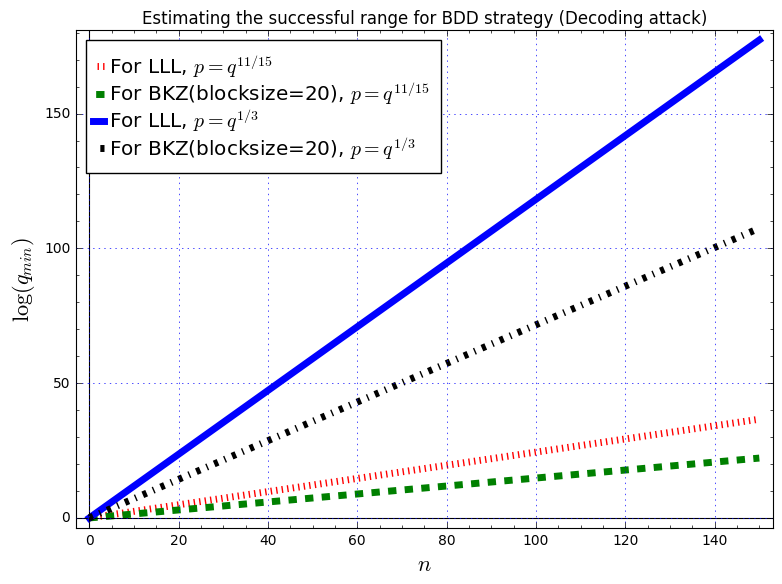
\includegraphics[scale=0.437, bb=0 0 560 430]{picture.png}
	\caption{We plot the graphs of the lines $\log (q_{\text{min}})=\lceil-4n  \log (c_{\mathcal{A}})/\zeta^2 \rceil$ corresponding to $\zeta=11/15$ and $\zeta=1/3$. For LLL, we use $c_{\text{LLL}}=0.9775$ and for BKZ of blocksize $20$ we use $c_{\text{BKZ}}=0.9868$.}
	\label{fig:success_range}
\end{figure}
%=======================
\paragraph{The Optimal Number of LWR Samples for the Decoding Attack}
%=======================
The optimal number of LWR samples $m$ should be chosen such that the right-hand side of
$2\sigma \leq c_{\mathcal{A}} ^{m} q^{\frac{m-n}{m}}$ is maximum.
So the optimal value of $m$ should be:
\begin{equation}\label{eq12} 
m=\left \lfloor \sqrt{\frac{n\log (q)}{- \log (c_{\mathcal{A}})}} \right\rceil.
\end{equation}
Remind that, the optimal number of samples typically used in attacking LWE problems (e.g., see \cite{LP11}, \cite{MR09}) is
%\begin{equation}\label{eq123} 
$m=\left \lfloor \sqrt{n\log (q)/\log (\delta_{\mathcal{A}})} \right\rceil,$
%\end{equation}
%====================
which along with Eq. \eqref{eq12} again convince us that $\delta_{\mathcal{A}} \approx 1/c_{\mathcal{A}}$ (see Subsection \ref{sec2.2}).

\section{Modulus Switching  on LWE and LWR} \label{sec5}
%====================

\subsection{Modulus Switching  on LWE }


Let $(\mathbf{a},c=\langle \mathbf{a},\mathbf{s}\rangle+e  \text{ mod } q) \in \mathbb{Z}_q^n \times \mathbb{Z}_q$ be an LWE modulo $q$ sample where $\mathbf{s}$ follows some distribution $\chi_s$ of variance $\sigma_s^2$ and the secret $e$ is sampled from a distribution of variance $\sigma_{lwe}^2$. Using the modulus switching, we consider the LWE instance $(\tilde{\mathbf{a}},\tilde{c}):=(\lfloor (q'/q).\mathbf{a}\rceil,\lfloor(q'/q).c \rceil) \in \mathbb{Z}_{q'}^n \times \mathbb{Z}_{q'}$ where we can write $\tilde{c}$ as 
$\tilde{c}=\left\langle \left\lfloor \tilde{\mathbf{a}} \right\rceil, \mathbf{s}\right\rangle \text{ mod } q'+\tilde{e},$
with $\tilde{e}:=e_2+(q'/q).e+e_3$, $e_2:=\left\langle (q'/q) \mathbf{a}-\left\lfloor (q'/q) \mathbf{a} \right\rceil, \mathbf{s}\right\rangle \text{ mod } q'$ and $ e_3 \in (-1/2,1/2]$. The variance of $e_3$ is $\sigma_3^2=1/12$ . The variance $\sigma^2_2$ of $e_2$ can be approximated as sum of $n$ summands in which each summand is uniform on $(-\sigma_s/2,\sigma_s/2]$ where $\sigma_s$ is the variance of the secret $\mathbf{s}$. Hence  $\sigma^2_2=n\sigma^2_s/12.$ 
Assume that $e_2, e_3$ and $(q'/q)\cdot e$ are three independent random variables,  the variance of $\tilde{e}$ can be estimated as 
\begin{equation}\label{keylwe}
{\sigma'}_{lwe}^2=\frac{(n\sigma_s^2+1)}{12}+\frac{\sigma_{lwe}^2}{q^2} q'^2\approx \frac{1}{12}(M_{lwe}q'^2+N),
\end{equation} with $M_{lwe}=12\sigma_{lwe}^2/q^2 $ and $N=n\sigma_s^2$. Particularly, if $\chi_e =\mathcal{D}_{\mathbb{Z},\alpha q}$ then $\sigma_{lwe}^2=\alpha^2 q^2/(2 \pi)$ and $M_{lwe}=6\alpha^2/\pi$.


Recall that, in the literature,  one typically chooses $q'$ such  that $\left\vert e_2 \right \vert \approx (q'/q)|e|$ yielding $$ q' \approx \frac{\sigma_{\mathbf{s}}}{\sigma_{lwe}}\sqrt{\frac{n}{12}}q$$ (cf. \cite{APS15}).

%=======================
\subsection{Modulus Switching on LWR}
%=======================


We will analyze the so-called \textit{$q'$-reduction} which reduces an LWR$_{m,n,q,p, \chi_s}$ instance to an LWE modulo $q'$ instance. Let
$(\mathbf{a}, c=\left\lfloor \langle \mathbf{a},\mathbf{s} \rangle \right\rceil_{q,p}) \in \mathbb{Z}_q^{n} \times \mathbb{Z}_p$  be an LWR sample. We reduce this LWR sample to the LWE sample modulo $q'$ of the form $(\mathbf{a}',c'=\langle \mathbf{a}',\mathbf{s} \rangle+e') \in \mathbb{Z}_{q'}^{n} \times \mathbb{Z}_{q'}$ with
$
c'=\left \lfloor (q'/q) \cdot c \right \rceil
$ clarified below
where $\mathbf{a}'=\left\lfloor (q'/q)\cdot \mathbf{a} \right\rceil$. We call the error $e'$ $q'$-\textit{error}. We now take a closer look into the process of generating $e'$. Recall that,
$c=\lfloor \langle \mathbf{a}, \mathbf{s} \rangle \rceil_{q,p} =({p}/{q})\cdot \langle \mathbf{a}, \mathbf{s} \rangle+p\cdot u+e_1$
for some $u\in \mathbb{Z}$, where $e_1 \leftarrow (1/q)\times \mathcal{U} \left(T \right )$ with $T=\{-\lfloor q/2 \rfloor,\cdots,\lfloor q/2 \rfloor \}$ (see Eq. \eqref{eq4} and the proof of Theorem \ref{theo1}).


Now with the $q'$-reduction we will obtain
\begin{equation*}
c_2:=\frac{q'}{p}\cdot c=\left \langle \left \lfloor \frac{q'}{q}\mathbf{a} \right \rceil, \mathbf{s} \right\rangle +\left \langle \frac{q'}{q} \mathbf{a}-  \left \lfloor \frac{q'}{q} \mathbf{a}\right \rceil , \mathbf{s} \right\rangle +q'\cdot u+e_4,
\end{equation*}
where $e_4:=(q'/p)\cdot e_1 \leftarrow q'/(pq) \cdot  \mathcal{U}(T),$ with $e_1$ as in Eq. \eqref{eq4}. Hence
\begin{equation*}
\begin{split}
c':&=\lfloor c_2 \rceil \text{ mod }q'\\
&=\left \langle \left \lfloor \frac{q'}{q}\mathbf{a} \right \rceil, \mathbf{s} \right\rangle \text{ mod }q' +\left \langle \frac{q'}{q} \mathbf{a}-  \left \lfloor \frac{q'}{q} \mathbf{a}\right \rceil , \mathbf{s} \right\rangle +e_4+e_6,
\end{split}
\end{equation*}
where $e_6 \in[-{1/2}, {1/2} ).$ The $q'$-error is 
$e':=e_4+e_5+e_6,$
with $e_5:=\left \langle (q'/q) \mathbf{a}-  \left \lfloor (q'/q) \mathbf{a}\right \rceil , \mathbf{s} \right\rangle$. 

\subsubsection{Distribution of $q'$-Error $e'$} 
The behaviour of the $q'$-error is mainly affected by that of $e_4$ (following a uniform distribution (cf. Section \ref{sec3})) and $e_5$ (following a Gaussian distribution via Central Limit Theorem (cf. \cite[Lemma 2]{APS15})). Then, using the Eq.  \eqref{keycon} on the convolution of two distributions, the probability density function of $e'$ can be approximated by
\begin{equation*}\label{keypdf}
\begin{split}
f(y)&=\frac{p\sqrt{6}}{q'\sqrt{\pi n \sigma_s ^2}} \int_{-\frac{q'}{2p}}^{\frac{q'}{2p}}\exp\left(-\frac{6(x-y)^2}{n\sigma_s^2}\right)dx\\
&=\frac{p}{q'\sqrt{\pi}}\int_ {\frac{\sqrt{6} \left(-\frac{q'}{2p}-y \right)}{{\sqrt{n}\sigma_s}}}^ {\frac{\sqrt{6} \left(\frac{q'}{2p}-y \right)}{{\sqrt{n}\sigma_s}}} \exp(-\zeta^2)d\zeta\\
&=\frac{p}{2q'} \cdot \left[\mathrm{erf} \left( \frac{\sqrt{6} \left(\frac{q'}{2p}-y \right)}{\sqrt{n}\sigma_s} \right) +\mathrm{erf} \left( {\frac{\sqrt{6} \left(\frac{q'}{2p}+y \right)}{{\sqrt{n}\sigma_s}}} \right)\right].
\end{split}
\end{equation*}
Its derivative is \begin{equation*}\label{key22}
\begin{split}
f'(y)&=\frac{\sqrt{6}p}{2\sqrt{\pi n} q'\sigma_s} \times \\\
&\times \left[-\text{exp} \left( \frac{-6 \left(\frac{q'}{2p}-y \right)^2}{n\sigma^2_s} \right) +\text{exp} \left( \frac{-6 \left(\frac{q'}{2p}+y \right)^2}{n\sigma^2_s} \right) \right].
\end{split}
\end{equation*}



The function $f(y)$ is symmetric through origin and its graph is a convex bell-shaped curve reaching its highest value $h(q')=({p}/{q'}) \times \mathrm{erf} \left( (\sqrt{6}q')/(2p\sqrt{n}\sigma_s)\right)$ 
at $y=0$.
It is easy to see that the functions $f'(y)$ and $h(q')$ tend to 0 as $q'$ increases. Thus, if $q' \gg p$, the error $e'$ will tend to follow a uniform distribution. By contrast, when $q' \approx p$, the error $e'$ will tend to be distributed via a Gaussian distribution (see Figure \ref{h2} for an illustration). 

The behavior of the $q'$-error $e'$ is complex, therefore we cannot use Eq. \eqref{eq18} or Eq. \eqref{eqkk} to estimate the success probability of the  decoding  attack in solving the LWE modulo $q'$. Also, on the other hand, we cannot compare the success probability of the  decoding  attack on the LWE modulo $q'$ with that on the LWE modulo $q$ using the formula \eqref{eq18} or \eqref{eqkk}. This is why we need to use Heuristic 1 (see Subsection \ref{heu}).

	\begin{figure}
	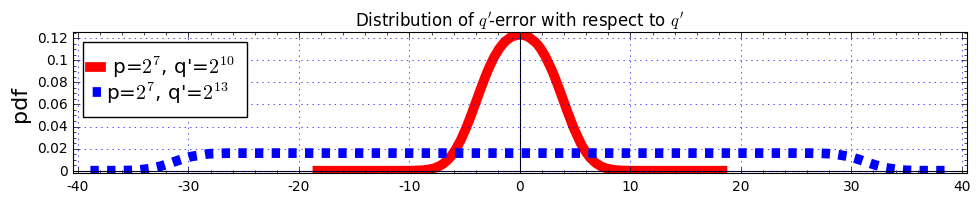
\includegraphics[scale=0.34]{error_distribution2.png}
	\caption{Distribution of the $q'$-error with respect to $q'$ given $p$. We consider two cases: $(p,q')=(2^7,2^{10})$ and $(p,q')=(2^7,2^{13})$ . In the first case, the graph of pdf is in bell shape like the graph of Gaussian pdf while in the second case the graph consists of a long straight segment in its middle. }
	\label{h2}
\end{figure}



\subsubsection {Variance of $q'$-Error}
We consider the variances of $e_4$, $e_5$ and $e_6$. The variance of $e_4$ will be
$$\sigma_4^2:=\left({q'^2}/{(q^2p^2)}\right)\cdot \left(\left(\left(2\lfloor q/2 \rfloor+1 \right)^2-1\right)/{12}\right).$$
Same as the case of LWE, we assume that $e_4, e_5$ and $e_6$ are three independent random variables, then the variance of $e'$ is estimated by
\begin{equation}\label{eq13}
\begin{split}
{\sigma'}_{lwr}^2& \approx \frac{1}{12} \left(n\sigma^2_s+\frac{q^2+2q}{q^2p^2}\cdot q'^2+1 \right)\\
&\approx \frac{1}{12} \left(M_{lwr} \cdot q'^2+N \right),
\end{split}
\end{equation}
where   $M_{lwr}:=(q^2+2q)/(p^2q^2)$ and $N:=n\sigma_s^2.$
Notice that, we can approximate 
\begin{equation}\label{eqmoi}
M_{lwr} \approx \frac{12\sigma_{lwr}^2}{q^2},
\end{equation}
with $\sigma_{lwr}^2$ as in Eq. \eqref{key}.

%=======================
\section {Known Attacks and Optimally Choosing  the Switching Modulo $q'$} \label{sec4}
%=======================

In this section, we will give the optimal formula for the switching modulus $q'$ according to each attack. Furthermore, we will also provide a corresponding sufficient condition under which one is able to decide whether one should use the modulus switching on the LWE/LWR instances or not. We focus on three typical attacks: the decoding  attack, the dual attack and the primal attack. 


\subsection{Our Framework and Notations}\label{sec41}
 For convenient, we will establish a common framework for both LWE and LWR under the modulus switching.  More specifically, we consider two LWE versions: one is the LWE modulo $q$, the other is the LWE modulo $q'$. The former is with respect to the original LWE modulo $q$ and the LWE modulo $q$ obtained from reducing LWR modulo $q$ to the LWE modulo $q$ without using the modulus switching. The latter is the LWE instance obtained by applying the modulus switching to the LWE modulo $q$ and to the LWR modulo $(q,p)$. More specifically,

\begin{itemize}
	\item \textit{Without the modulus switching:} In this case, the LWE modulo $q$  instance we deal with consists of $m$ LWE samples of the form $(\mathbf{a},c) \in \mathbb{Z}_q^{n} \times \mathbb{Z}_q$ where
	$c =\langle \mathbf{a}, \mathbf{s} \rangle \text{ mod } q+e$
	and the error $e$ has variance of $ \sigma^2$. We call each specific attack against this LWE instance \textit{the $q$-attack}, for instances the $q$-decoding attack, the $q$-dual attack and the $q$-primal attack.
	
	\item \textit{With the modulus switching:}  In this case, the LWE modulo $q'$ instance we deal with consists of $m$ LWE samples of the form $(\mathbf{a}',c') \in \mathbb{Z}_{q'}^{n} \times \mathbb{Z}_{q'}$
	where $c'=\langle \mathbf{a}',\mathbf{s} \rangle \text{ mod } q'+e'$ and $\mathbf{a}'=\left\lfloor ({q'}/{q}) \cdot \mathbf{a} \right\rceil,$ and the $q'$-error $e'$ has variance of  
	$\sigma'^2 =\left(Mq'^2+N \right)/12
	$.
	We call each specific attack against this LWE instance \textit{the $q'$-attack}, for instances the $q'$-decoding attack, the $q'$-dual attack and the $q'$-primal attack.
\end{itemize} 
%=======================
\begin{remark}  \label{rem2}
	%=======================	
From now on, we abuse the notations $M, N, \sigma, \sigma'$ without caring about which original problem (the LWE modulo $q$ or the LWR modulo $(q,p)$) we are dealing with. In particular, for LWR, we will replace $M=12\sigma^2/q^2$ with $M_{lwr}= 12 \sigma_{lwr}^2/q^2$, $\sigma^2$ with $\sigma_{lwr}^2= (q^2+2qp)/(12p^2)$ and ${\sigma'}^2$ with ${\sigma'}_{lwr}^2$ as in Eq. \eqref{eq13}. Likewise, for LWE, $M$ will be replaced with $M_{lwe}=12 \sigma_{lwe}^2/q^2$, $\sigma^2$ will be replaced with $\sigma_{lwe}^2$, and $\sigma'^2$ with ${\sigma'}_{lwe}^2$ as in Eq. \eqref{keylwe}. Still, $N=n\sigma_s^2$  is the same for both LWE and LWR.

\end{remark} 

In what follows, according to each attack, we try to choose $q'$ such that the $q'$-attack is ``\textit{optimal}'' in the sense that the success probability of this attack on LWE modulo $q'$ is highest. Then, we find a condition under which the $q'$-attack is more powerful than the $q$-attack.

We assume that the number of samples $m$ is kept the same for both the $q$-attack and the $q'$-attack.  Note that, for each attack, the optimal $m$ will be chosen corresponding to the LWE modulo $q$. Such a choice of $m$ will be theoretically optimal to the $q$-attack not the $q'$-attack. However, this implies that the $q'$-attack can be stronger if one appropriately choose for it the optimal $m$. 



%=======================
\subsection{The Decoding Attack}  \label{heu}
%=======================

The decoding attack proposed by Lindner and Peikert \cite{LP11} is based on the close relation between the search-LWE problem and the BDD problem. Given a lattice and a target vector \textit{unusually close} to the lattice, the BDD problem asks to find the lattice vector closest to the target. 

Let $(\mathbf{A}, \mathbf{c}=\mathbf{A}\mathbf{s}+\mathbf{e} \mod q) \in \mathbb{Z}_q^{m \times n} \times \mathbb{Z}_q^m$  be an LWE modulo $q$ instance. We set $$\Lambda_q{(\mathbf{A})}=\left\{ \mathbf{u} \in \mathbb{Z}^m: \mathbf{u}=\mathbf{A}\mathbf{s} \text{ mod } q \text{ for some } \mathbf{s} \in \mathbb{Z}^n \right\}$$ to be  the $q$-ary lattice spanned by columns of $\mathbf{A}$ and we call it \textit{the associated $q$-ary lattice} of the search-LWE problem $(\mathbf{A}, \mathbf{c})$. If the error $\mathbf{e}$ is sufficiently short then $\mathbf{c}$ is closest to some lattice point $\mathbf{u}=\mathbf{A}\mathbf{s} \text{ mod } q \in \Lambda_q(\mathbf{A})$ since we have $\mathbf{e}=\mathbf{c}-\mathbf{A}\mathbf{s}.$  Thus, finding the secret $\mathbf{s}$ is equivalent to finding $\mathbf{u}$, i.e., solving a CVP problem over $q$-ary lattice $\Lambda_q{(\mathbf{A})}$. The most basic tools used in solving search-LWE via the decoding attack are some basis reduction algorithm, say $\mathcal{A}$ (e.g., LLL or BKZ), and the Babai's Nearest Plane (BNP) algorithm. The BNP algorithm takes as input the vector  $\mathbf{c}$  and a basis $\mathbf{B}=\{ \mathbf{b}_1,\cdots,\mathbf{b}_{m}\}$ of  $\Lambda_q(\mathbf{A})$ that is already reduced by $\mathcal{A}$ and outputs the lattice point $\mathbf{u} \in \Lambda_q(\mathbf{A})$ such that $\mathbf{e}=\mathbf{c}-\mathbf{u} \in\mathcal{P}_{1/2}(\mathbf{B^*}) $. 

From now on, by ``the decoding attack'', we mean the  solving strategy associated with the BNP algorithm described above. Note also that, the decoding attack needs $m > n$, and the optimal $m$ is approximated by Eq. \eqref{eq12}.



\paragraph{The Decoding Attack and Root Hermite Factor} It is conventional that the quality of a reduced basis (which is characterized by the rHF obtained using by some LBR algorithm) has the most significant effect on the success probability of the BNP algorithm (see, e.g., \cite[Section 5.4]{APS15}, \cite{BBD+15, GvVW17}), hence the decoding attack. Namely, a smaller rHF means that the corresponding basis is reduced better, hence the BNP algorithm may return the closest vector more precisely, so the efficacy of the decoding attack may be higher.  Assume for example that the decoding attack deploys the LBR algorithm named $\mathcal{A}$.  Also, suppose that we want to compare the efficacy of the decoding attack in solving a search-LWE problem $(\mathbf{A}_1, \mathbf{c}_1)$ with that in solving a search-LWE problem  $(\mathbf{A}_2, \mathbf{c}_2)$. Then instead of success probability, we can compare the rHFs of $\mathcal{A}$ with respect to the reduced bases of the associated $q$-ary lattices $\Lambda_q{(\mathbf{A}_1)}$ and $\Lambda_q{(\mathbf{A}_2)}$.


%=======================
\paragraph{Success Probability of  the Decoding Attack} 
%=======================
The success probability of the decoding attack in solving search-LWE can be measured by the probability of the event that the error $\mathbf{e}$ lies in $\mathcal{P}_{1/2}(\mathbf{B^*})$.
Depending on which distribution the error $\mathbf{e}$ follows, we have some formulas to compute the probability in the literature: (i) if $\mathbf{e}$ is uniform then we can estimate the probability by
\begin{equation}\label{eq18}
\mathrm{Pr}\left[ \mathbf{e} \in \mathcal{P}_{1/2}(\mathbf{B^*})\right]= \prod_{i=1}^{m}\left(  \frac{ \rceil \Vert\mathbf{b}^{*}_i \Vert}{2\sigma_e\sqrt{3}} \right), 
\end{equation}
(ii) in the case of a Gaussian error $\mathbf{e}$, we can use the formula taken from \cite{LP11}
\begin{equation}\label{eqkk}
\mathrm{Pr}\left[ \mathbf{e} \in \mathcal{P}_{1/2}(\mathbf{B^*})\right]=\prod_{i=1}^{m}\mathrm{erf}\left( \frac{ \rceil \Vert \mathbf{b^{*}}_i \Vert}{2 \sigma_e \sqrt{2}} \right),
\end{equation} 
where $\sigma^2_e $ is the variance of the error $\mathbf{e}$ according to its distribution and $\mathrm{erf}(\cdot)$ is the Gaussian error function 
$$\mathrm{erf}(z)=\frac{2}{\sqrt{\pi}}\int_{0}^{z} \text{exp}(-t^2)dt, z \in [0, +\infty].$$
However, Eq. \eqref{eq18} and Eq. \eqref{eqkk} are really not helpful for our work. We cannot use either Eq. \eqref{eq18} or Eq. \eqref{eqkk} if the error $\mathbf{e}$ has a complex behavior. Such a kind of error is the $q'$-error that we saw in Section \ref{sec5}. Therefore, we have to look for another way to estimate the success probability for the  decoding attack regardless of the error's distribution. Fortunately, we can use a heuristic analysis appeared in \cite{KYGY16} as follows:

We have $$\mathrm{Pr}\left[ \mathbf{e} \in \mathcal{P}_{1/2}(\mathbf{B^*})\right]=\mathrm{Pr}\left[\vert \langle \mathbf{e}, \mathbf{b}_i^{*} \rangle \vert < \frac{\Vert \mathbf{b}_i^{*} \Vert^2}{2}, \forall i=1,\cdots,m\right].$$ 
Using the heuristics that
$\vert \langle \mathbf{e}, \mathbf{b}_i^{*} \rangle \vert  \approx \Vert \mathbf{e} \Vert \cdot \Vert \mathbf{b}_i^{*} \Vert /\sqrt{m}$ and  $\Vert \mathbf{e} \Vert \approx \sigma_e \cdot \sqrt{m}$, we have  $2 \sigma_e \leq \Vert \mathbf{b}_i^{*} \Vert \text{ for all } i=1,\cdots,m,$ which is equivalent to 
\begin{equation}\label{keym}
2 \sigma_e \leq \min_{i=1,\cdots,m}\Vert \mathbf{b}_i^* \Vert.
\end{equation}
Combining Eq. \eqref{keym} with Eq. \eqref{eq1} yields the following heuristic that will be very useful for our analysis on the decoding attack:
%=======================
\paragraph{Heuristic 1} 
%=======================
\textit{Let $c_{\mathcal{A}}$ is defined as in Eq. \eqref{eq1}. Heuristically, the success probability for the decoding attack in solving search-LWE problem $(\mathbf{A}, \mathbf{c}=\mathbf{A}\mathbf{s}+\mathbf{e} \mod q) \in \mathbb{Z}_q^{m \times n} \times \mathbb{Z}_q^m$ can be measured by the probability
	$\mathrm{Pr}\left[2\sigma_e \leq c_{\mathcal{A}}^m \cdot \det(\Lambda_q{(\mathbf{A})})^{1/m}\right],$
	namely,
	$\mathrm{Pr}\left[2\sigma_e \leq c_{\mathcal{A}}^m \cdot q^{(m-n)/m}\right]$,
	which is equivalent to
	\begin{equation*}\label{eqa}
	\mathrm{Pr} \left[\frac{q^{m-n}}{\sigma_e^m} \geq  \frac{2^m}{c_{\mathcal{A}}^{m^2}}\right],
	\end{equation*}
	where $\mathcal{A}$ is the LBR algorithm used within the decoding attack.}



According to the heuristic, the success probability of the $q$-decoding attack is
\begin{equation*}\label{keyw}
\mathrm{Pr} \left[\frac{q^{m-n}}{\sigma^m} \geq  \frac{2^m}{c_{\mathcal{A}}^{m^2}}\right].
\end{equation*}
Similarly, that of the $q'$-decoding attack is
\begin{equation*}\label{keya}
\mathrm{Pr} \left[\frac{q'^{m-n}}{\sigma'^m} \geq  \frac{2^m}{c_{\mathcal{A}}^{m^2}}\right].
\end{equation*}
Set $P':=q'^{m-n}/ \sigma'^m $ and $ P:= q^{m-n}/ \sigma^m$. Our goal is to choose $q'$ maximizing $P'$ and with the chosen $q'$, we check the condition when $P' \geq P$. In other words, we choose $q'$ such that
\begin{equation*}\label{eqn}
P' \text{ is maximum, (denote } P'_{\text{max}}),
\end{equation*} 
and $P'_{\text{max}} \geq P$.
The condition $P' \geq P$ is equivalent to
\begin{equation}\label{eqk1}
\frac{q'^{m-n}\cdot \sqrt{12^m}}{\sqrt{(Mq'^2+N)^m}} \geq \frac{q^{m-n}}{\sigma^m}.
\end{equation}

Now, it is the time to state the main result for applying the modulus switching to the decoding attack.

\begin{theorem} \label{theorem3} Let $m, n, M, N, q, q', \sigma, \sigma', \sigma_s$ as mentioned in Subsection \ref{sec41} and required that $m>n$. Assume that we apply the modulus switching technique to the decoding attack against the LWE/LWR problems. Then
	
	(i) The optimal switching modulus $q'$ for the decoding attack is
	\begin{equation} \label{eq26}
	q' \approx \sqrt{\frac{(m-n)N}{nM}}.
	\end{equation}
	
	(ii) The $q'$-decoding attack is stronger than the $q$-decoding attack if the following sufficient condition holds: 
		\begin{equation}\label{key6}
	\left(\frac{12\sigma^2}{\sigma_s^2}\right)^{n} \geq\frac{m^m}{(m-n)^{m-n}}.
		\end{equation}

\end{theorem}
\begin{proof}

It is easy to see that $q'= \sqrt{(m-n)N/(nM)}$ maximizes $h(q'):=q'^{m-n}\sqrt{12^m}/\sqrt{(Mq'^2+N)^m}$. Then the maximum of $h(q')$ is 

$$\sqrt{\frac{(m-n)^{m-n} \cdot n^n \cdot 12^m}{m^m \cdot N^n \cdot M^{m-n}}}.$$
After some calculations, we get from Eq. \eqref{eqk1} that 
\begin{equation}\label{key1}
	\left(\frac{12\sigma^2}{m}\right)^{m} \geq \left( \frac{N}{n}\right)^{n} \cdot \left(\frac{ q^{2} \cdot M}{m-n} \right)^{m-n}.
\end{equation}
By Remark \ref{rem2} and some arrangements, Eq. \eqref{key1} can be rewritten as Eq. \eqref{key6}.

\end{proof}

\begin{remark}
We remark that the statement (ii) of Theorem \ref{theorem3} differs from \cite[Theorem 2 (ii)]{LMDY18}. In the effort of simplifying the Eq. \eqref{key1},  we made a mistake to claim in the proof of \cite[Theorem 2 (ii)]{LMDY18} that the function $x \ln(x)$ is concave over $(0,+\infty)$. Actually, that claim is  not correct and simplifying is unnecessary. In the proof for Theorem \ref{theorem3} (ii) of the present paper, we do not use that claim and only transform Eq. \eqref{key1} into Eq. \eqref{key6} using Remark \ref{rem2}.
\end{remark}
\subsection{The Dual Attack}\label{dualattack}
The dual attack aims to solving the decision version of LWE and LWR.  Namely, to distinguish an LWE instance   $(\mathbf{A}, \mathbf{c}) \in \mathbb{Z}_q^{m \times n} \times \mathbb{Z}_q^m$ with the uniform $(\mathbf{A}, \mathbf{c}) \in \mathbb{Z}_q^{m \times n} \times \mathbb{Z}_q^m$, the attacker considers the $q$-ary lattice
\begin{equation*}\label{dualla}
\Lambda_q^{\bot}{(\mathbf{A})}=\left\{ (\mathbf{x}, \mathbf{y}) \in \mathbb{Z}^m \times \mathbb{Z}^n:\mathbf{x}^t\cdot \mathbf{A}=\mathbf{y}^t \text{ mod } q \right\},
\end{equation*}
and then uses an LBR algorithm,  again named $\mathcal{A}$,  to get a reduced basis of the lattice and then get a short vector, let's say $\mathbf{u}_0=(\mathbf{x}_0, \mathbf{y}_0)$. Notice that if $(\mathbf{A}, \mathbf{c})$ is uniform then 
\begin{equation*}\label{keypp}
z:=\langle \mathbf{x}_0, \mathbf{c}\rangle=\langle \mathbf{y}_0, \mathbf{s}\rangle+\langle \mathbf{x}_0, \mathbf{e}\rangle \text{ mod } q
\end{equation*}
is also uniform modulo $q$. By contrast, if $(\mathbf{A}, \mathbf{c})$ is LWE, i.e., we have $ \mathbf{c}= \mathbf{A}\cdot \mathbf{s}+ \mathbf{e} \text{ mod } q$ then $z$ tends to be distributed via a Gaussian distribution of mean $0$ and its variance $\sigma_z^2\approx \Vert \mathbf{u}_0\Vert^2\sigma^2$ as $n$ increases, where $\sigma^2$ is the variance of the error $\mathbf{e}$. This suggests the attacker to check whether the value $z$ is small or not. 

A reasoning in \cite[Section 6.4]{ADP+11} says that the dual attack has the distinguishing advantage upper bounded by $4 \text{exp}(-2\pi^2\sigma_z^2/q^2)=4 \text{exp}(-2\pi^2\Vert \mathbf{u}_{0}\Vert^2\sigma^2/q^2)$. As a result, the success probability of the dual attack depends heavily on the quantity $\Vert \mathbf{u}_0\Vert\sigma/q$. The smaller quantity is better for the dual attack. Assume that we try to exploit the modulus switching technique in the dual attack. We should choose the new modulus $q'$ such that the quantity is smallest. 

Now we give more details.

\begin{itemize}
	\item \textit{In the $q$-dual attack:} The error $\mathbf{e}$ has the variance $\sigma^2$. Since we can estimate $\Vert \mathbf{u}_0\Vert\approx {\delta_{\mathcal{A}}}^{m+n}q^{n/(m+n)}$ by Eq.  \eqref{keyk}, we have $$\frac{\Vert \mathbf{u}_0\Vert\sigma}{q}=\frac{{\delta_{\mathcal{A}}}^{m+n}q^{n/(m+n)}{\sigma}}{q}.$$
	
	\item\textit{ In the $q'$-dual attack:} The corresponding error $\mathbf{e'}$ has the variance $\sigma'^2=(M{q'}^2+N)/12$. Same as above, we can estimate $\Vert \mathbf{u}'_{0}\Vert\approx {\delta_{\mathcal{A}}}^{m+n}{q'}^{n/(m+n)}$, hence
	$$\frac{\Vert \mathbf{u}'_{0}\Vert\sigma'}{q'}=\frac{1}{\sqrt{12}}{\delta_{\mathcal{A}}}^{m+n}{q'}^{\frac{-m}{m+n}}\sqrt{M{q'}^2+N}.$$
\end{itemize}

We come to the following theorem for the dual attack giving the optimal switching modulus optimal  and a condition to efficiently exploit the modulus switching technique in this attack.
\begin{theorem} \label{theorem4} Let $m, n, M, N, q, q', \sigma, \sigma', \sigma_s$ as mentioned in Subsection \ref{sec41}. Assume that we apply the modulus switching technique to the dual attack against the LWE/LWR problems. Then
	
	(i) The optimal switching modulus $q'$ for the dual attack is
	\begin{equation} \label{eqmm}
	q'\approx \sqrt{\frac{mN}{nM}}.
	\end{equation}
	
	(ii) The $q'$-dual attack is stronger than the $q$-dual attack if the following sufficient condition holds:
		\begin{equation}\label{keym4}
	\left(\frac{12\sigma^2}{\sigma_s^2}\right)^{n} \geq\frac{(m+n)^{m+n}}{m^{m}}.
\end{equation}
	%In other words, the sufficient condition is that
	%$q'^{\text{opt}} \leq \sqrt{\frac{m-n}{n}}\cdot q$.}
\end{theorem}
\begin{proof}
We should choose  $q'$ such that $g(q'):={q'}^{\frac{-m}{m+n}}\sqrt{M{q'}^2+N}$ is minimum. It is easy to see that such a $q'$ is $$q'=\sqrt{\frac{mN}{nM}}.$$ Then the minimum of $g(q')$ is $$\sqrt{\left(\frac{mN}{nM}\right)^{-\frac{m}{m+n}} \cdot \frac{(m+n)N}{n}}.$$
Now, we suppose that $\Vert \mathbf{v'}_{0}\Vert\sigma'/q' \leq \Vert \mathbf{v}_{0}\Vert\sigma/q$, which is equivalent to
$$ \left(\frac{mN}{nM}\right)^{-\frac{m}{m+n}} \cdot \frac{(m+n)N}{n}.\frac{1}{12} \leq \frac{q^{2n/(m+n)}{\sigma^2}}{q^2},$$
i.e.,
\begin{equation*}\label{eqwm}
\left(\frac{12\sigma^2}{m+n}\right)^{m+n} \geq \left( \frac{N}{n}\right)^{n} \cdot \left(\frac{ q^{2} \cdot M}{m} \right)^m,
\end{equation*}
which can be rewritten as
Eq. \eqref{keym4} using Remark \ref{rem2}.

% \begin{equation*}\label{key12}
%\left(\frac{12\sigma^2}{\sigma_s^2}\right)^{n} %\geq\frac{(m+n)^{m+n}}{m^{m}}.
%\end{equation*}
\end{proof}


\begin{remark}
We can see that differing from the decoding attack, we do not need $m>n$ but the arbitrary integer $m>0$. We also can choose the optimal $m$ for the dual attack by finding $m$ minimizing the quantity ${\delta_{\mathcal{A}}}^{m+n}q^{n/(m+n)}$ given $n, q, \delta_{\mathcal{A}}$. Namely, 
\begin{equation}\label{eqtt} 
m=\left \lfloor \sqrt{\frac{n\log (q)}{\log (\delta_{\mathcal{A}})}} \right\rceil-n.
\end{equation}

\end{remark}

\subsection{The Primal Attack}\label{primalattack}
The primal attack solves the search-LWE problem by transforming the problem into an Unique Shortest Vector Problem (uSVP). Let $\gamma>1$ be a real number, the uSVP$_{\gamma}$ problem is to find the shortest non-zero vector of a lattice $\mathcal{L}$ given that the gap $\lambda_2(\mathcal{L})/\lambda_1(\mathcal{L})\geq\gamma$. It is folklore that the bigger the gap $\lambda_2(\mathcal{L})/\lambda_1(\mathcal{L})$ is, the easier the uSVP is. (See more discussions in \cite{AFG14, GN08}.) 


 Let  $(\mathbf{A}, \mathbf{c}=\mathbf{A}\cdot \mathbf{s}+\mathbf{e}) \in \mathbb{Z}_q^{m \times n} \times \mathbb{Z}_q^m$ be an LWE instance, we have $\mathbf{A}\cdot \mathbf{s}+\mathbf{e}-\mathbf{c}=\mathbf{0} \text{ mod } q$.
Consider the $q$-ary lattice 
\begin{equation*}\label{primalla}
\Lambda=\left\{ \mathbf{v} \in \mathbb{Z}^{n+m+1}:(\mathbf{A}| \mathbf{I}_m|-\mathbf{c})\mathbf{v}=\mathbf{0} \text{ mod } q \right\}.
\end{equation*}
Then $\mathbf{v}_0=(\mathbf{s}| \mathbf{e}|\mathbf{1})$ will be an unusual short vector in the lattice if $\mathbf{s}$ and $\mathbf{e}$ are short. It is known that if the gap between two minima $\lambda_2(\Lambda)$ and $\lambda_1(\Lambda)$ is sufficiently large then the short vector $\mathbf{v}_0$ may be found using an LBR algorithm. Recall that we can estimate $\lambda_2(\Lambda)=\sqrt{(m+n+1)/(2 \pi \mathfrak{e})}\cdot q^{\frac{m}{m+n+1}}$ by Gaussian Heuristic, whereas $\lambda_1(\Lambda)=\Vert (\mathbf{s}| \mathbf{e}|\mathbf{1}) \Vert=\sqrt{\Vert \mathbf{s}\Vert^2+\Vert \mathbf{e}\Vert^2+1}\approx \sqrt{n\sigma_s^2+1+m\sigma^2}\approx \sqrt{N+m\sigma^2}$. %Again, we let $N:=n\sigma_s^2+1, M=\frac{6\alpha^2}{\pi}.$ 

Now if we use the modulus switching technique on the LWE, we attain a new LWE instance $(\mathbf{A'}, \mathbf{c'}=\mathbf{A'}\cdot \mathbf{s}+\mathbf{e'}) \in \mathbb{Z}_{q'}^{m \times n} \times \mathbb{Z}_{q'}^m$ where $\mathbf{A}'=\left\lfloor ({q'}/{q}) \cdot \mathbf{A} \right\rceil,$ hence a corresponding $q'$-ary lattice. 
$$\Lambda'=\left\{ \mathbf{v'} \in \mathbb{Z}^{n+m+1}:(\mathbf{A'}| \mathbf{I}_m|-\mathbf{c'})\mathbf{v'}=\mathbf{0} \text{ mod } q' \right\}.$$
Same as above, the shortest vector of the $q'$-ary lattice is $\mathbf{v'}_0=(\mathbf{s}| \mathbf{e'}|\mathbf{1})$. Accordingly, $\lambda_2(\Lambda')=\sqrt{(m+n+1)/(2 \pi \mathfrak{e})}\cdot {q'}^{\frac{m}{m+n+1}}$ and 
\begin{align*}
\lambda_1(\Lambda')&=\Vert (\mathbf{s}| \mathbf{e'}|\mathbf{1}) \Vert=\sqrt{\Vert \mathbf{s}\Vert^2+\Vert \mathbf{e'}\Vert^2+1}\\
&\approx \sqrt{n\sigma_s^2+m\sigma'^2}=\sqrt{Pq'^2+Q},
\end{align*}
where 
\begin{align}\label{keypq}
 Q=(m+12)N/12,\sigma'^2=(Mq'^2+N)/12, P=mM/12.
\end{align}

We have the following theorem:
\begin{theorem} \label{theorem5} Let $m, n, M, N, q, q', \sigma, \sigma', \sigma_s$ as mentioned in Subsection \ref{sec41}. Assume that we apply the modulus switching technique to the primal attack against the LWE/LWR problems. Then
	
	(i) The optimal switching modulus $q'$ for the primal attack is
	\begin{equation} \label{eqm}
	q'\approx \sqrt{\frac{(m+12)N}{(n+1)M}}.
	\end{equation}
	
	(ii) The $q'$-primal attack is stronger than the $q$-primal attack if the following sufficient condition holds:  
		
		
		\begin{equation}\label{keya4}
			\left(\frac{12(N+m\sigma^2)}{m+n+1}\right)^{m+n+1} \geq \left( \frac{(m+12)N}{n+1}\right)^{n+1} \cdot \left( q^{2} M \right)^{m}.
			\end{equation}	
			
\end{theorem}

\begin{proof}
We will choose $q'$ optimal such that the ratio 
$$\frac{\lambda_2(\Lambda')}{\lambda_1(\Lambda')}=\frac{\sqrt{\frac{m+n+1}{2 \pi \mathfrak{e}}}\cdot {q'}^{\frac{m}{m+n+1}}}{\sqrt{Pq'^2+Q}},$$
is maximum, i.e., the function $f(q'):=\frac{ {q'}^{\frac{m}{m+n+1}}}{\sqrt{Pq'^2+Q}}$ is maximum. It is easy to obtain that such a $q'$ is
$$q'=\sqrt{\frac{yQ}{(1-y)P}}=\sqrt{\frac{(m+12)N}{(n+1)M}},$$  with $y:=\frac{m}{m+n+1}$
and the maximum of $f(q')$ is $$\sqrt{\frac{y^y Q^{y-1}}{(1-y)^{y-1}P^{y}}}.$$


Now, we need $$\max\left(\frac{\lambda_2(\Lambda')}{\lambda_1(\Lambda')} \right)\geq \frac{\lambda_2(\Lambda)}{\lambda_1(\Lambda)},$$  which is
\begin{equation*}
\begin{split}
&\frac{(n+1)^{n+1} \cdot 12^{m+n+1}}{(m+n+1)^{m+n+1} \cdot (m+12)^{n+1}\cdot N^{n+1}\cdot M^m}\\
& \geq \frac{q^{2m}}{(N+m\sigma^2)^{m+n+1}},\\
\end{split}
\end{equation*}
equivalently,
\begin{equation*}\label{keymn}
\left(\frac{12(N+m\sigma^2)}{m+n+1}\right)^{m+n+1} \geq \left( \frac{(m+12)N}{n+1}\right)^{n+1} \cdot \left( q^{2} M \right)^{m}.
\end{equation*}
\end{proof}
\begin{remark}
Same as the dual attack, we do not need $m>n$. And we can choose the optimal $m$ satisfying that $ 
m+n+1=\left \lfloor \sqrt{\frac{n\log (q)}{ \log (\delta_{\mathcal{A}})}} \right\rceil,$
i.e., 
\begin{equation}\label{eqtt2} 
m=\left \lfloor \sqrt{\frac{n\log (q)}{\log (\delta_{\mathcal{A}})}} \right\rceil-n-1,
\end{equation}
by using the arguments in \cite[Section 4.2]{BG14}.
\end{remark}
%======================
\section{The Modulus Switching vesus the Rescaling } \label{modvsre}
%======================
In this section, we will revisit the dual attack and the primal attack that were presented in Subsection \ref{dualattack} and Subsection \ref{primalattack}. However, we will focus only on the LWE instances  $(\mathbf{A}, \mathbf{c}=\mathbf{A}\cdot \mathbf{s}+\mathbf{e}) \in \mathbb{Z}_q^{m \times n} \times \mathbb{Z}_q^m$ whose $\Vert \mathbf{s}\Vert \ll \Vert \mathbf{e} \Vert$. As we will see later in Section \ref{sec8}, Round5 \cite{BBGM+19} and SABER \cite{DKRV19} are two NIST PQC submissions having this characteristic. 
We will compare the efficacy of the so-called rescaling technique to that of the modulus switching on these attacks. The main idea of the rescaling technique that was proposed in \cite[Subsection 6.1]{BG14} and further analyzed in \cite{CKLS16, BBGM+19} is to re-balance the contributions of summands relating to the secret and the error in the corresponding context of each attack. As we will see below, this technique changes the volume of the lattice (due to the change of the modulus), and also slightly changes the norm of the shortest vector in the corresponding CVP instance. One expects that the Hermite factor of the problem might be increased and if so the successful range of the lattice attack is widened. That is why the rescaling technique is also considered as a technical solution to enhance the power of the lattice attacks.  Apparently, the technique looks like the same as the modulus switching technique. Therefore, we will consider in details the rescaling technique applied to the dual attack and the primal attack and then have a comparison between these two techniques to get a condition under which the modulus switching is better than the rescaling. For convenient, we also refer all notations to  Section \ref{sec4}.
 
\paragraph{The Dual Attack}
For the dual attack, using the rescaling technique, instead of the lattice as in Subsection \ref{dualla}, we construct the following alternative lattice of the form:
\begin{equation*}\label{dualre}
\Lambda_{\omega}{(\mathbf{A})}=\left\{ \left(\mathbf{x}, \frac{\mathbf{y}}{\omega}\right) \in \mathbb{Z}^m \times \frac{1}{\omega}\cdot \mathbb{Z}^n:\mathbf{x}^t\cdot \mathbf{A}=\mathbf{y}^t \text{ mod } q \right\}.
\end{equation*}
We call $\omega$ \textit{the rescaling factor}. Define $q_{\omega}=q/\omega$, then $\text{vol}(\Lambda_{\omega}{(\mathbf{A})})=q_{\omega}^{n}$. Using an LBR algorithm $\mathcal{A}$ of the root Hermite Factor $\delta_{\mathcal{A} }$, we can find the short vector of the form $\mathbf{u}_{0, {\omega}}=(\mathbf{x}_0, \mathbf{y}_0/\omega) \in \Lambda_{\omega}{(\mathbf{A})}$
and $\Vert \mathbf{u}_{0, {\omega}}\Vert\approx {\delta_{\mathcal{A}}}^{m+n}(q_{\omega})^{n/(m+n)}$. The rescaling factor
$\omega$ will be chosen to equalize the contribution of $\mathbf{s}$ and $\mathbf{e}$, namely we can choose $\omega=\sigma/\sigma_s$. Then
$z:=\langle \mathbf{x}_0, \mathbf{c}\rangle=\langle \mathbf{y}_0, \omega \mathbf{s}\rangle+\langle \mathbf{x}_0, \mathbf{e}\rangle \text{ mod } q$. Again, we pay our attention to the quantity
$$\frac{\Vert \mathbf{u}_{0, {\omega}}\Vert \sigma}{q}=\frac{{\delta_{\mathcal{A}}}^{m+n}q_{\omega}^{n/(m+n)}{\sigma}}{q}.$$


Recall that, in the case of using the modulus switching with the modulus $q'$, we have
$$\frac{\Vert \mathbf{u}'_{0}\Vert\sigma'}{q'}=\frac{1}{\sqrt{12}}\cdot {\delta_{\mathcal{A}}}^{m+n}{q'}^{\frac{-m}{m+n}}\sqrt{M{q'}^2+N},$$ 
which is minimum of  $\frac{1}{\sqrt{12}}\cdot {\delta_{\mathcal{A}}}^{m+n}\sqrt{\left(\frac{mN}{nM}\right)^{-\frac{m}{m+n}} \cdot \frac{(m+n)N}{n}}$ at  $q'=\sqrt{mN/(nM)}.$


So as to compare the modulus switching with the rescaling, we compare $\Vert \mathbf{u}_{0, {\omega}}\Vert \sigma/q$ with $\Vert \mathbf{u}'_{0}\Vert\sigma'/q'$: Assume that the former is bigger than the latter (i.e., the modulus switching is better than the rescaling), we have
$$q_{\omega}^{n/(m+n)}\frac{\sigma}{q} \geq \frac{1}{\sqrt{12}}\sqrt{\left(\frac{mN}{nM}\right)^{-\frac{m}{m+n}} \cdot \frac{(m+n)N}{n}}.$$
Simplifying the above equation, we attain
\begin{equation*}\label{eqwmw}
	\left(\frac{12}{m+n}\right)^{m+n} \cdot \sigma^{2m} \cdot \sigma_s^{2n} \geq \left( \frac{N}{n}\right)^{n} \cdot \left(\frac{ q^{2} \cdot M}{m} \right)^m,
	\end{equation*}
	i.e.,
	\begin{equation*}\label{key4}
	\left(\frac{12\sigma^2}{\sigma_s^2}\right)^{n} \geq\frac{(m+n)^{m+n}}{m^{m}}\cdot \frac{\sigma^{2n}}{\sigma_s^{2(m+n)}}.
\end{equation*}



\paragraph{The Primal Attack} \label{primalre}
For this attack, using the rescaling technique, we construct the following lattice instead of the lattice as in Subsection \ref{primalla}:
\begin{equation*}\label{primallan}
L_{\omega}=\left\{ \mathbf{v}_{\omega} \in \mathbb{Z}^{n+m+1}:(\mathbf{A}| \omega\mathbf{I}_m|-\mathbf{c})\mathbf{v}_{\omega}=\mathbf{0} \text{ mod } q \right\},
\end{equation*}
with $\omega=\sigma/\sigma_s$. Then $\mathbf{v}_{0, {\omega}}=(\mathbf{s}| \omega^{-1}\cdot \mathbf{e}|\mathbf{1})$ will be an unusual short vector in $L_{\omega}$. Set $q_{\omega}:=\omega^{-1}q$, then we have $\lambda_2(L_{\omega})=\sqrt{\frac{m+n+1}{2 \pi \mathfrak{e}}}\cdot q_{\omega}^{\frac{m}{m+n+1}}$ and $\lambda_1(L_{\omega})=\Vert \mathbf{v}_{0, {\omega}} \Vert=\sqrt{N+m\sigma_s^2}$.


Again, if we use the modulus switching, we get the $q'$-ary lattice
$$L'=\left\{ \mathbf{v'} \in \mathbb{Z}^{n+m+1}:(\mathbf{A'}| \mathbf{I}_m|-\mathbf{c'})\mathbf{v'}=\mathbf{0} \text{ mod } q' \right\},$$
with $\mathbf{A}'=\left\lfloor ({q'}/{q}) \cdot \mathbf{A} \right\rceil,$
and $\lambda_2(L')=\sqrt{\frac{m+n+1}{2 \pi \mathfrak{e}}}\cdot {q'}^{\frac{m}{m+n+1}}$, $
\lambda_1(L')\approx \sqrt{Pq'^2+Q}, $
where $\sigma'^2, P$, and $Q$ as in Eq. \eqref{keypq}.

We compare the modulus switching with the rescaling by determining when the condition $ \lambda_2(L')/\lambda_1(L') \geq \lambda_2(L_{\omega})/\lambda_1(L_{\omega})$ holds (i.e., when the modulus switching is better than the rescaling), which is equivalent to
\begin{equation*}
\begin{split}
&\frac{(n+1)^{n+1} \cdot 12^{m+n+1}}{(m+n+1)^{m+n+1} \cdot (m+12)^{n+1}\cdot N^{n+1}\cdot M^m} \\
&\geq \frac{q_{\omega}^{2m}}{(N+m\sigma_s^2)^{m+n+1}}.
\end{split}
\end{equation*}
Simplyfing the equation we obtain,
	\begin{equation*}\label{keymnn}
\begin{split}
&\left(\frac{12(N+m\sigma^2)}{m+n+1}\right)^{m+n+1}\\
& \geq \left( \frac{(m+12)N}{n+1}\right)^{n+1} \cdot \left( q^{2} M \right)^{m} \cdot \frac{\sigma_s^{2m}}{\sigma^{2m}} .
\end{split}
\end{equation*}

To summary, we have the following theorem:


\begin{theorem}[Modulus Switching vs Rescaling] Let $m$, $n$, $M$, $N$, $q$, $q'$, $\sigma$, $\sigma_s$ as mentioned in Subsection \ref{sec41}.
	
	(i) For the dual attack, the modulus switching outperforms the rescaling technique if the following requirement holds
	\begin{equation}\label{eqwmwq}
		\left(\frac{12\sigma^2}{\sigma_s^2}\right)^{n} \geq\frac{(m+n)^{m+n}}{m^{m}}\cdot \frac{\sigma^{2n}}{\sigma_s^{2(m+n)}}.
		\end{equation}
	
	(ii) For the primal attack, the modulus switching outperforms the rescaling technique if the following requirement holds
	
		\begin{equation}\label{keymn2n}
		\begin{split}
&\left(\frac{12(N+m\sigma^2)}{m+n+1}\right)^{m+n+1}\\
& \geq \left( \frac{(m+12)N}{n+1}\right)^{n+1} \cdot \left( q^{2} M \right)^{m} \cdot \frac{\sigma_s^{2m}}{\sigma^{2m}} .
\end{split}
	\end{equation}
\end{theorem}

\begin{remark}
Considering Eq. \eqref{keymn2n} together with Eq. \eqref{keya4}, we can see in the case $\sigma_s<\sigma$ that if Eq. \eqref{keya4} holds we will also have Eq. \eqref{keymn2n} to hold. This turns out that for the primal attack against LWE/LWR instances, if we can apply the modulus switching to it (i.e., Eq. \eqref{keya4} holds) then the modulus switching is a better than the  rescaling. However, for the dual attack, the relation between Eq. \eqref{eqwmwq} and Eq. \eqref{keym4} is not clear since when $\sigma_s<\sigma$ we still do not whether   $\sigma^{2n}/\sigma_s^{2(m+n)}$ is larger than 1 or not. In the case that the ratio is smaller than 1 and Eq. \eqref{keym4} holds, for the dual attack against LWE/LWR instances, if we are able to use modulus switching (i.e., Eq. \eqref{keym4} holds) then the modulus switching is a better choice rather than the rescaling technique. 
Take SABER \cite{DKRV19} as an example, with the proposed parameters $\sigma_s$, $\sigma$ and $m=n$  (see Table \ref{tab9}) we have $\sigma^{2n}/\sigma_s^{2(m+n)}<1$. Thus using the modulus switching technique is better rather than the rescaling technique in the dual attack against SABER.
\end{remark}



\begin{table}[pt]
	\centering
	\small\addtolength{\tabcolsep}{1.7pt}
	\caption{\textbf{How to choose parameters and proceed with our experiments\\ in Section \ref{sec6}?} } 
	
	\begin{tabular}{p{8cm}}
		
		\hline
		\hline
		
		1. First, we choose $\zeta$. The first $\zeta=11/15$ is inspired from choosing parameters in the work of \cite{BBGM+19}, the last one $\zeta=1/3$ comes from  \cite{DTV15} whilst two middle ones $\zeta=2/3$ and $\zeta=1/2$ are additionally suggested by us.  Then choose $n$ and compute $\log (q_{\text{min}})$ by \eqref{eq11} (for the decoding attack). We focus on $n=60, n=80$ and $n=100$.\\
		2. Next, choose $\log (q)$ to be around $\log (q_{\text{min}})$ (in the case of the decoding attack), from which we have $q$ and $p$.
		After that we compute $q'$ by \eqref{eq26}.\\
		3. Choose $m$: For the decoding attack, we compute $m$ by \eqref{eq12}, while for the primal attack we choose $m$ by \eqref{eqtt2}.  \\
		4. With chosen parameters, we check the condition \eqref{key6} or the condition \eqref{keya4} depending on the attack we are considering. \\
		5. For each tuple ($\zeta, n, q, p, q'$), we sample 10 LWR instances. The small secret $\mathbf{s}$ is drawn uniformly at random over $\{-1,0,1\}^n$.\\
		6. For each LWR instance, transform it to the LWE modulo $q$ and the LWE modulo $q'$. \\
		7. Finally, run the attacks on these two LWE instances. \\
		\hline
		\hline
		
	\end{tabular}
	\label{table:1}
\end{table}


%======================================
\section{The Impact of the Modulus Switching on the Rescaling} \label{impact}
%======================================

Again, in this section, we consider the LWE modulo $q$ instances   $(\mathbf{A}, \mathbf{c}=\mathbf{A}\cdot \mathbf{s}+\mathbf{e}) \in \mathbb{Z}_q^{m \times n} \times \mathbb{Z}_q^m$  whose $\Vert \mathbf{s}\Vert \ll \Vert \mathbf{e} \Vert$ and only focus on the dual attack and the primal attack. For convenient, we also refer all notations to  Sections \ref{sec4} and \ref{modvsre}. Assume that we perform the modulus switching with the switching modulus $q'$ first and then we apply the rescaling technique on the LWE instance. We will show that such a combination of these two techniques will make both the dual attack and the primal attack worse. Stress that the same phenomenon was reported by Bai and Galbraith in \cite{BG14}  for the primal attack. However, we will base our work  on new theoretical arguments other than that of \cite{BG14}. 





\paragraph{The Dual Attack}


For the dual attack, first we do the modulus switching to reduce the LWE/LWR problem modulo $q$ to the LWE problem modulo $q'=\sqrt{mN/(nM)} $, and then we do the rescaling on the new LWE modulo $q'$ with the rescaling factor 
$$\omega_{\text{mod}}=\frac{\sigma'}{\sigma_s}=\sqrt{\frac{Mq'^2+N}{12\sigma_s^2}},$$ where $\sigma'$ is the standard deviation of the $q'$-error (see Subsection \ref{sec41}).  
Then the resulting lattice $\Lambda_{\text{mod,}\omega}{(\mathbf{A}')}$, which is

\begin{equation*}\label{dualreq}
\left\{ \left(\mathbf{x}, \frac{\mathbf{y}}{\omega_{\text{mod}}}\right) \in \mathbb{Z}^m \times \frac{1}{\omega_{\text{mod}}}\cdot \mathbb{Z}^n:\mathbf{x}^t\cdot \mathbf{A}'=\mathbf{y}^t \text{ mod } q' \right\}
\end{equation*}
with $\mathbf{A}'=\left\lfloor ({q'}/{q}) \cdot \mathbf{A} \right\rceil$, has volume of $q_{\text{mod}}^n$ with $$q_{\text{mod}}:=\omega_{\text{mod}}^{-1}\cdot q'=\frac{q'\cdot \sigma_s}{\sigma'}.$$ 


Sames as the arguments in Subsection \ref{dualre}, we can find the short vector $\mathbf{u}_{0,\text{mod}, {\omega}}\in \Lambda_{\text{mod,}\omega}$ using an LBR algorithm $\mathcal{A}$ of the root Hermite Factor $\delta_{\mathcal{A} }$ and by Gaussian Heuristic we have
\begin{equation*}
\begin{split}
\frac{\Vert \mathbf{u}_{0,\text{mod}, {\omega}}\Vert\sigma'}{q'}&=
{\delta_{\mathcal{A}}}^{m+n}\cdot \frac{{q_{\text{mod}}}^{\frac{n}{m+n}}\cdot \sigma'}{q'}\\
&={\delta_{\mathcal{A}}}^{m+n}\cdot \left(\frac{\sigma'}{q'}\right)^{\frac{m}{m+n}}\sigma_s^{\frac{n}{m+n}},
\end{split}
\end{equation*}
while only exploiting the rescaling without the modulus switching we get the short vector $\mathbf{u}_{0, {\omega}}=
{\delta_{\mathcal{A}}}^{m+n}\cdot q_{\omega}^{\frac{n}{m+n}}.$ Hence

$$\frac{\Vert \mathbf{u}_{0, {\omega}}\Vert\sigma}{q}=
{\delta_{\mathcal{A}}}^{m+n}\cdot \frac{q_{\omega}^{\frac{n}{m+n}}\cdot \sigma}{q}={\delta_{\mathcal{A}}}^{m+n}\cdot \left(\frac{\sigma}{q}\right)^{\frac{m}{m+n}}\sigma_s^{\frac{n}{m+n}}.$$

Again, thus, we just need to compare $\frac{\sigma'}{q'}$ with $\frac{\sigma}{q}$. We have  $$\frac{\sigma'}{q'}=\frac{Mq'^2+N}{12q'}=\sqrt{\frac{(m+n)M}{12m}}> \sqrt{\frac{M}{12}} = \frac{\sigma}{q},$$
yielding that 
$$\frac{\Vert \mathbf{u}_{0,\text{mod}, {\omega}}\Vert\sigma'}{q'} \geq \frac{\Vert \mathbf{u}_{0, {\omega}}\Vert\sigma}{q}.$$
This claims that if we use the modulus switching first and we apply the rescaling alter, then the dual attack will be weaker than the dual attack only using the rescaling. 
\paragraph{The Primal Attack}


For the primal attack, only using the rescaling technique we have
\begin{align*}
\frac{\lambda_2(L_{\omega})}{\lambda_1(L_{\omega})}&=\frac{\sqrt{\frac{m+n+1}{2 \pi  \mathfrak{e}}}\cdot {q_{\omega}}^{\frac{m}{m+n+1}}}{\sqrt{N+m\sigma_s^2}},
\end{align*}
with $\omega=\sigma_s/\sigma$  and $q_{\omega}=q/\omega=q\sigma_s/\sigma$ as in Section \ref{modvsre}.

Now, assume that first we do the modulus switching to reduce the LWE/LWR problem modulo $q$ to the LWE problem modulo $q'=\sqrt{(m+12)N/((n+1)M)}$ , and then the rescaling is performed on the new LWE modulo $q'$ with the rescaling factor 
$$\omega_{\text{mod}}=\frac{\sigma'}{\sigma_s}=\sqrt{\frac{Mq'^2+N}{12\sigma_s^2}},$$ where $\sigma'$ is the standard deviation of the $q'$-error (cf. Subsection \ref{sec41}).  
Then the resulting lattice $L_{\text{mod,}\omega}$, which is

\begin{equation*}\label{primallanpq}
\left\{ \mathbf{v}_{\text{mod},\omega} \in \mathbb{Z}^{n+m+1}:(\mathbf{A}'| \omega_{\text{mod}}\mathbf{I}_m|-\mathbf{c})\mathbf{v}_{\text{mod},\omega}=\mathbf{0} \text{ mod } q' \right\}
\end{equation*}
with $\mathbf{A}'=\left\lfloor ({q'}/{q}) \cdot \mathbf{A} \right\rceil$, has volume of $q_{\text{mod}}^n$ with $$q_{\text{mod}}:=\omega_{\text{mod}}^{-1}\cdot q'=\sigma_s\cdot \sqrt{\frac{12(m+12)}{(m+n+13)M}}.$$
Since $12/M=q^2/\sigma^2$, we have
\begin{equation}\label{keymm}
q_{\text{mod}}=\frac{q\cdot\sigma_s}{\sigma}\cdot \sqrt{\frac{m+12}{m+n+13}} < \frac{q\cdot\sigma_s}{\sigma}=q_{\omega}.
\end{equation}
 Observe that $\mathbf{v}_{0, \text{mod},{\omega}}:=(\mathbf{s}| \omega_{\text{mod}}^{-1}\cdot \mathbf{e}'|\mathbf{1})$ will be an unusual short vector in $L_{\text{mod},\omega}$. Thus $\lambda_1(L_{\text{mod,}\omega})=\lambda_1(L_{\omega})=\sqrt{N+m\sigma_s^2}$.
 Then 
\begin{align*}
\frac{\lambda_2(L_{\text{mod,}\omega})}{\lambda_1(L_{\text{mod,}\omega})}=\frac{\sqrt{\frac{m+n+1}{2 \pi  \mathfrak{e}}}\cdot {q_{\text{mod}}}^{\frac{m}{m+n+1}}}{\sqrt{N+m\sigma_s^2}}.
\end{align*}


Due to Eq. \eqref{keymm}, we obtain \begin{align*}
\frac{\lambda_2(L_{\text{mod,}\omega})}{\lambda_1(L_{\text{mod,}\omega})}
&\leq \frac{\sqrt{\frac{m+n+1}{2 \pi  \mathfrak{e}}}\cdot {q_{\omega}}^{\frac{m}{m+n+1}}}{\sqrt{N+m\sigma_s^2}}=\frac{\lambda_2(L_{\omega})}{\lambda_1(L_{\omega})}.
\end{align*}

 The result in this subsection again confirms the observation of \cite{BG14} that using the modulus switching (in which they chose $q'/q\approx 1/8$ (cf. \cite[Section 5]{BG14}) before performing their attack (which is the same as the primal attack accompanied by the rescaling technique) will make the attack worse.



%======================
\section{Implementation and Experimental Results} \label{sec6}
%======================
We implemented the decoding attack and the primal attack on LWR problem to evaluate the efficacy of the $q'$-attack in comparison with the $q$-attack. In our experiments, we used SageMath version 8.1 \cite{Sag81} to implement these two attacks. The LBR algorithm used in our experiments is LLL \cite{LLL82}. We used the  function``.LLL()''  to call the floating point implementation of LLL in the \textit{fplll} library which is included in SageMath with the default reduction parameter $0.99$. By using such an LLL algorithm, we have the corresponding constant mentioned in Eq. \eqref{eq1} is $c_{\text{LLL}}=0.9775$ (see Section \ref{sec2.2}). 




%=======================


The experimental results are summarized in Tables \ref{table:2} - \ref{table:6}.  We refer to Table \ref{table:1} for generating parameters, sampling LWR instances, as well as how to run attacks on the corresponding LWE instances.

We highlight some noticeable things from our experimental results:
\begin{itemize}
	\item For the decoding attack, in all cases, the rHF of the $q$-attack is always bigger than that of the $q'$-attack. Interestingly, the rHF of the $q'$-attack becomes smaller once $\zeta$ declines while the rHF of the $q$-attack does not seem to change, namely, rHF$(q') \approx 1.0201$ for all considered $\zeta$'s. Recall that, smaller root Hermite factor means that the LWE modulo $q'$ instance is more easily solved by attacks than the LWE modulo $q$ instance (see Subsection \ref{heu}). For the primal attack, the case of $\zeta=11/15$, sometimes we have  rHF($q'$) $>$rHF($q$).
	\item When $\zeta$ is close to $1$, such as $\zeta=11/15$, the $q'$-attack does not outperform the $q$-attack much. In contrast, when $\zeta$ is closer to 0 than 1, e.g., $\zeta=1/3$,  $q'$ approach is much efficient than the $q$-attack in terms of success probability, rHF and even running time (we add the runtime data in Table \ref{table:6} ) since $q'$ is quite close to $p$ and smaller than $q$.
	% For example, with $\zeta=1/3, n=100$, we $\log (q')=59$ that is much less than $\log (q)=119$.
	\item The bit size $\log(q')$ is quite close to $\log(p)$. Namely, in all considered cases, we have $\log(q')-\log(p)$ equals to $3$ \text{ or } $4$. It seems that the difference $\log(q')-\log(p)$ increases (but slowly) once either $n$ increases or/and $\zeta$ decreases.  
	
\end{itemize}



\begin{table*}[t]
	\caption{ \textbf{We compare $q'$-decoding attack with $q$-decoding attack against LWR:} $\zeta$ is the bit ratio of $p$ and $q$, i.e., $\zeta=\log (p)/ \log (q)$; $n$ is the dimension of the secret; $\log (q_{\text{min}})$ is the smallest bit size of $q$ computed by \eqref{eq11} given $\zeta$, $n$; $\log (q')$, $\log (q)$, $\log(p)$ are the bit size of the modulus $q'$ computed by Eq. \eqref{eq26}, of moduli $q$ and $p$, respectively; $m$ is the optimal number of LWR samples for the decoding  attack computed by Eq. \eqref{eq12} (we use the same number of samples $m$ in both the $q$-decoding attack and $q'$-decoding attack); the columns entitled ``succ($q$)'', ``succ($q'$)'',  ``rHF($q$)'' and ``rHF($q'$)'' represent the success probability of the $q$-decoding attack and of the $q'$-decoding attack, the rHF's of the $q$-attack and of the $q'$-attack, respectively. Note that, rHF($q$) and rHF($q'$) are computed using Eq. \eqref{eq1}. We did not count the running ttime for this experiment.  We ran this experiment on a MacBook Pro (Retina, 13-inch, Early 2015) installing macOS High Sierra version 10.13.3 with Memory 8GiB 1867 MHz DDR3, Processor 2.7GHz Intel Core i5, Graphics Intel Iris Graphics 6100 1536 MB.} 
	\centering
	\small\addtolength{\tabcolsep}{0pt}
	
	\begin{tabular}{| c|| c|c | c | c | c | c | c |c|c| c| c|}	
		\hline
		\hline
		\multirow{2}{*}{$\zeta$}&\multicolumn{4}{c|}{LWR parameters ($p=q^{\zeta}$)}& Switching modulus&\multicolumn{2}{c|}{Success Probability}&\multicolumn{2}{c|}{Root Hermite Factor}&Satifying\\
		&$(n, \log (q_{\text{min}}))$& $\  m\ $& $\log (q)$ & $\log (p)$  & $\log (q')$ & succ($q$) & succ($q'$)&rHF$(q)$&rHF$(q')$&Eq. \eqref{key6}\\
		\hline
		\hline
		
		\multirow{8}{*}{$\frac{11}{15}$}&(60,15)&166&\textbf{15}&11&\textbf{14}&\textbf{0\%}&\textbf{60\%}&1.0202&1.0200&Y\\
		
		&(60,15) &176&\textbf{17}&12&\textbf{15}&\textbf{100\%}&\textbf{100\%}&1.0203&1.0197&Y\\
		
		&	(80,20)&204&\textbf{17}&12&\textbf{15}&\textbf{0\%}&\textbf{0\%}&1.0209&1.0200&Y\\
		
		&(80,20)&209&\textbf{18}&13&\textbf{16}&\textbf{20\%}&\textbf{80\%}&1.0205&1.0200&Y\\
		
		&(80,20)&221&\textbf{20}&15&\textbf{19}&\textbf{80\%}&\textbf{100\%}&1.0209&1.0200&Y\\
		
		&(80,20)&232&\textbf{22}&16&\textbf{20}&\textbf{100\%}&\textbf{100\%}&1.0205&1.0200&Y\\
		
		
		&(100,25)&247&\textbf{20}&15&\textbf{19}&\textbf{20\%}&\textbf{60\%}&1.0210&1.0203&Y\\
		
		
		&(100,25)&276&\textbf{25}&18&\textbf{22}&\textbf{100\%}&\textbf{100\%}&1.0212&1.0195&Y\\
		
		
		\hline
		
		
		\multirow{9}{*}{$\frac{2}{3}$}&(60,18)&171&\textbf{16}&11&\textbf{14}&\textbf{80\%}&\textbf{80\%}&1.0203& 1.0199&Y\\	
		
		
		
		&(60,18)&176&\textbf{17}&11&\textbf{14}&\textbf{20\%}&\textbf{60\% }&1.0201&1.0188&Y\\	
		&(60,18)&181&\textbf{18}&12&\textbf{15}&\textbf{100\%}&\textbf{100\% }&1.0202&1.0191&Y\\		
		
		&(80,24)&226&\textbf{21}&14&\textbf{18}&\textbf{20\%}&\textbf{100\%}&1.0203&1.0187&Y\\	
		&(80,24)&237&\textbf{23}&15&\textbf{19}&\textbf{40\%}&\textbf{100\% }&1.0215&1.0180&Y\\	
		&(80,24)&242&\textbf{24}&16&\textbf{20}&\textbf{100\%}&\textbf{100\% }&1.0208&1.0183&Y\\		
		
		&(100,30)&270&\textbf{24}&16&\textbf{20}&\textbf{0\%}&\textbf{80\% }&1.0211&1.0184&Y\\
		
		&(100,30)&281&\textbf{26}&17&\textbf{21}&\textbf{0\%}&\textbf{100\% }&1.0211&1.0179&Y\\
		&(100,30)&292&\textbf{28}&19&\textbf{23}&\textbf{100\%}&\textbf{100\%} &1.0213&1.0182&Y\\	
		
		\hline	
		
	
		
		
			\multirow{3}{*}{$\frac{1}{3}$}&(60,71)	&299&\textbf{49}&16&\textbf{20}&\textbf{0\%}&\textbf{100\% }&1.0215&1.0091&Y\\	
		
		&(80,95)&386&\textbf{61}&20&\textbf{24}&\textbf{0\%}&\textbf{100\% }&1.0214&1.0088&Y\\		
		&(100,119)&424&\textbf{59}&20&\textbf{24}&\textbf{0\%}&\textbf{100\% }&1.0213&1.0091&Y\\	
		
		\hline	
		
		\multirow{6}{*}{$\frac{1}{2}$}&(60,32)&218&\textbf{26}&13&\textbf{17}&\textbf{0\%}&\textbf{100\%}&1.0210&1.0142&Y \\			
		&(60,32)&234&\textbf{30}&15&\textbf{19}&\textbf{20\%}&\textbf{100\%} &1.0201&1.0140&Y\\	
		
		&80,43)&256&\textbf{27}&14&\textbf{18}&\textbf{0\%}&\textbf{80\% }&1.0208&1.0146&Y\\
		&80,43)&292&\textbf{35}&18&\textbf{22}&\textbf{0\%}&\textbf{100\% }&1.0209&1.0140&Y\\
		
		
		&(100,53)&307&\textbf{31}&16&\textbf{20}&\textbf{0\%}&\textbf{60\%} &1.0214&1.0143&Y\\
		&(100,53)&336&\textbf{37}&19&\textbf{23}&\textbf{0\%}&\textbf{100\%} &1.0213&1.0138&Y\\		
		\hline
	\end{tabular}
	\label{table:2}
	
\end{table*}





\begin{table*}[t]
	%\centering
	\caption{\textbf{We compare the $q'$-primal attack with the $q$-primal attack against LWR:} Notations are same as in Table \ref{table:2}. We note some more things: $\log (q')$ is the bit size of the modulus $q'$ computed by Eq. \eqref{eqm}, $m$ is the optimal number of LWR samples for the primal attack computed by Eq. \eqref{eqtt} (we use the same number of samples $m$ in both the $q$-primal attack and the $q'$- primal attack); the columns entitled  ``time($q'$)'' represent the running time of  the $q$-primal attack and of the $q'$-primal attack (in seconds), respectively. The last column is to check the condition in Eq. \eqref{keya4}: ``Y'' means the condition is satisfied while ``N'' means not. We ran this experiment on a desktop computer installing Ubuntu 16.04 LTS, with Memory 15.7GiB, Processor Intel Core i7 CPU870@2.93Ghz $\times$ 8, Graphics NVA8.}
	\small\addtolength{\tabcolsep}{-2pt}
	\begin{tabular}{| c|| c| c | c | c | c || c | c |c|c| c|c|c| }
		
		\hline
		\hline
		\multirow{2}{*}{$\zeta$}&\multicolumn{4}{c|}{LWR parameters ($p=q^{\zeta}$)}&Switching modulus&\multicolumn{2}{c|}{Success Probability}&\multicolumn{2}{c|}{Root Hermite Factor}&\multicolumn{2}{c|}{Running time}&Satisfying\\
		&$n$& $m$& $\log (q)$ & $\log (p)$  & $\log (q')$  & succ($q$) & succ($q'$)&rHF$(q)$&rHF$(q')$&time$(q)$&time$(q')$&Eq. \eqref{keya4}\\
		\hline
		\hline
		
		\multirow{4}{*}{$\frac{1}{2}$}&60&131&\textbf{20}&10&\textbf{14}&\textbf{0\%}&\textbf{80\%}&0.9869&0.9787&17961 sec& 9093 sec &Y\\			
		&80&176&\textbf{27}&14&\textbf{18}&\textbf{0\%}&\textbf{60\% }&1.0213&0.9832&146812 sec&68110 sec&Y\\
		
		
		&100&202&\textbf{30}&15&\textbf{19}&\textbf{0\%}&\textbf{40\%}&1.0203&0.9854&506745 sec&240675 sec&Y\\
		&100&217&\textbf{33}&17&\textbf{21}&\textbf{0\%}&\textbf{80\%}&1.0201&0.9825&534835 sec&304330 sec&Y\\
		
		
		\hline
		
		\multirow{3}{*}{$\frac{2}{3}$}&60&111&\textbf{16}&11&\textbf{14}&\textbf{80\%}&\textbf{100\%}&0.9876&0.9839&11436 sec&6397 sec&Y\\
		
		&80&135&\textbf{19}&13&\textbf{17}&\textbf{60\%}&\textbf{100\%}&0.9869&0.9850&52615 sec&38645 sec&Y\\
		
		&100&165&\textbf{23}&15&\textbf{19}&\textbf{20\%}&\textbf{100\%}&0.9857&0.9834&336873 sec&245531 sec&Y\\
		
		
		\hline
		
		\multirow{6}{*}{$\frac{11}{15}$}&60&36&\textbf{5}&4&\textbf{7}&\textbf{0\%}&\textbf{0\%}&1.0185&1.0189&56 sec&76 sec&N\\
		&60&94&\textbf{13}&10&\textbf{13}&\textbf{20\%}&\textbf{60\%}&0.9854&0.9869&3957 sec&3900 sec&Y\\
		
		
		&80&117&\textbf{16}&12&\textbf{15}&\textbf{60\%}&\textbf{80 \%}&0.9867&0.9868& 26448 sec& 24014 sec&Y\\
		
		
		&100&23&\textbf{5}&4&\textbf{6}&\textbf{0\%}&\textbf{0\%}&1.0152&1.0159&62 sec&77 sec&N\\
		&100&147&\textbf{20}&15&\textbf{19}&\textbf{0\%}&\textbf{80\%}&0.9859&0.9849&144161 sec&120588 sec&Y\\
		
		
		&	100&114&\textbf{15}&11&\textbf{14}&\textbf{0\%}&\textbf{0\%}&1.0152&1.0159&62 sec&77 sec&N\\
		
		
		\hline
		
		
		
	\end{tabular}
	\label{table:6}
\end{table*}




%===============
\section{Accessing the Impact of Modulus Switching on LWE/LWR-based Round 2 NIST PQC Submissions} \label{sec8}
%===============
Among 17 public-key encryption and key-establishment schemes and 9 digital signature schemes that was released as candidates for the second round NIST PQC Standardization, there are up to 9 submissions based on LWE/ LWR variants \cite{AAA+19}. Each candidate proposes some tuples of parameters fulfilling one or more target security categories. In this section, we first give some more necessary notions and then review all the LWE/LWR-based second round submissions and try to check whether or not we should apply the modulus switching to them.

First, we give the definition of the centered binomial distribution (see, for example, \cite[Section 2.4 ]{LLJ+19} or \cite[Section 2.1]{DKRV19}). The distribution is used in some NIST PQC Submissions as an alternative to the Gaussian sampling which is costly to implement in practice  and also impacted by the side channel attacks.

\begin{definition}[Centered Binomial Distribution]
The centered binomial distribution of parameter $\eta$, denoted as $\Psi_\eta$,  samples two bits $a$ and $b$ from the binary set $\{0,1\}$ then outputs $a-b$ with the following condition: the probability of the output $0$ is $(2-\eta)/2$ and the probability of each of the outputs $1, -1$ is $\eta/4$. The standard deviation of this distribution is $\sqrt{\eta/2}$.
\end{definition}

LAC \cite{LLJ+19} with its latest version submitted to the second round NIST PQC submission changes to exploit the so-called \textit{fixed weight centered binomial distribution} in which the Hamming weight of a random vector following the distribution is fixed. 
\begin{definition}[Fixed Weight Centered Binomial Distribution] \label{fix}
	The fixed weight centered binomial distribution of parameter $(\eta, n, h)$ is a $n$-ary centered binomial distribution, denoted as $\Psi_\eta^{n,h}$ when ($0<h<n/2$), outputs trinary vectors of length $n$ whose the number of is $1$ and of $-1$ is $h/2$, respectively, and the number of $0$ is $n-h$. The standard deviation of this distribution is $\sqrt{h/n}$ and also is equal to $\sqrt{\eta/2}$ .
\end{definition}



\begin{figure}[pt]
	\centering
	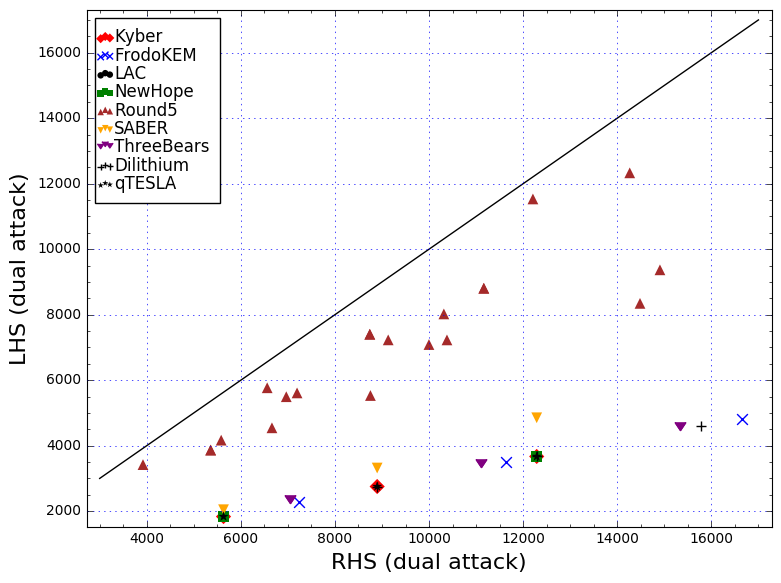
\includegraphics[scale=0.445, bb=0 0 560 430]{nist2.png}
	\caption{Using data in Table \ref{tab9}, we evaluate the impact of the modulus switching again the second round NIST PQC Submissions under the dual attack. ``LHS'', ``RHS'' mean the left-hand side and the right-hand side, respectively, of Eq. \eqref{keym4}. The line represents the case of the equality LHS$=$RHS. A point which is over the line means that an instance of the corresponding submission will be affected by the modulus switching.  We see that all points are under the line, so the modulus switching is not available to apply to the dual attack in breaking the hard underlying problems of the NIST PQC submissions listed in Section \ref{sec8} with proposed parameters.}
	\label{fig:nist2}
\end{figure}

\begin{figure}[pt]
	\centering
	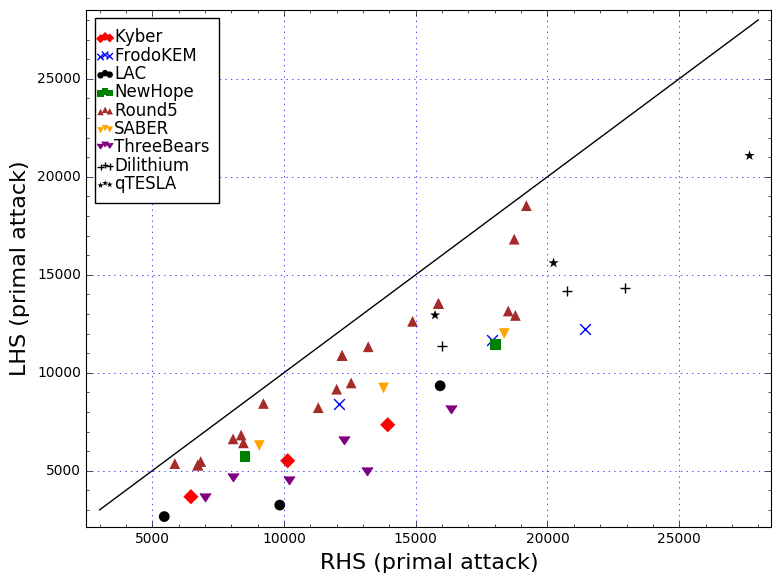
\includegraphics[scale=0.445, bb=0 0 560 430]{nist1.png}
	\caption{Same as Figure \ref{fig:nist2}, except that we consider Eq. \eqref{keya4} with respect to the primal  attack. }
	\label{fig:nist1}
\end{figure}


Besides LWE and LWR, many NIST PQC submissions also base their security on other algebraic variants of LWE and LWR, namely Ring-LWE/Ring-LWR (RLWE/RLWR), Module-LWE/Module-LWR (MLWE/MLWR), or even an integer variant of MLWE called ILWE.
 In these variants, instead of vectors, one uses a number of polynomials drawn from some polynomial ring \cite{LPR10}. Specifically, we usually consider the ring $R_q:=\mathbb{Z}_q[x]/ \langle x^n+1\rangle,$ where $n$ is power of two. 

 So far, there has been no special attacks that exploit the algebraic structure of these variants. The typical way to attack these algebraic instances is to consider them as ``standard'' LWE/LWR instances in which a polynomial can be considered as a vector of its coefficients and a product of two polynomials can be represented as a matrix-vector multiplication. By ``standard'' LWE/LWR we mean the LWE/LWR problems defined as in Subsection \ref{lwer}.
Formally, we will give some more definitions below. Here, let $\chi_s$ and $\chi_e$ be distributions over $R_q$. 
%The hardness of the RLWE is based on that of the lattice problems over ideal lattices rather than random lattices which LWE bases on.
%=======================
\begin{definition}[RLWE Problems]
	%=======================
	Given an RLWE  instance $(a,c=a \cdot s+e) \in  R_q \times  R_q$ where $a \leftarrow \mathcal{U}(R_q)$, $s \leftarrow \chi_s$ and $e \leftarrow \chi_e$:
	\begin{itemize}
		\item The search-RLWE (sRLWE) problem is to find the secret $s$.
		\item The decision-RLWE (dRLWE) problem requires to distinguish the RLWE instance  from the uniform pair $(a,c)\in  R_q \times  R_q$.
	\end{itemize}
\end{definition}


%=======================
\begin{definition}[MLWE Problems]
	%=======================
	Given an MLWE instance $(\mathbf{A},\mathbf{c}=\mathbf{A} \cdot \mathbf{s}+\mathbf{e}) \in  R_q^{m\times n} \times  R_q^{m}$ where $\mathbf{A} \leftarrow \mathcal{U}(R_q^{m \times n})$, $\mathbf{s} \leftarrow \chi_s^n$ and $\mathbf{e} \leftarrow \chi_e^m$:
	\begin{itemize}
		\item The search-MLWE (sMLWE) problem is to find the secret $\mathbf{s}$.
		\item The decision-MLWE (dMLWE) problem requires to distinguish the MLWE instance  from the uniform pair $(\mathbf{A},\mathbf{c}) \in  R_q^{m\times n} \times  R_q^{m}$.
	\end{itemize}
\end{definition}
	 
	 
	 
	 
	 
	 %=======================
	 \begin{definition}[RLWR Problems] 
	 	%=======================
	 	Given an RLWR  instance   $(a,c=\lfloor a \cdot s \rceil_{q,p}) \in R_q \times R_p$, where $a \leftarrow \mathcal{U}(R_q)$, and $s\leftarrow \chi_s$:
	 	\begin{itemize}
	 		\item  The search-RLWR (sLWR) problem is to find the secret $\mathbf{s}$. 
	 		\item The decision-RLWR (dLWR) problem requires to distinguish the ring-LWR instance from the uniform pair $(a,c)\in  R_q \times  R_p$.
	 	\end{itemize}
	 \end{definition}
	 
	 
	 
	 %=======================
	 \begin{definition}[MLWR Problems] 
	 	%=======================
	 	Given an MLWR  instance   $(\mathbf{A},\mathbf{c}=\lfloor \mathbf{A}\mathbf{s}  \rceil_{q,p}) \in R_q^{m \times n} \times R_p^m$, where $\mathbf{A} \leftarrow \mathcal{U}(R_q^{m \times n})$, and $\mathbf{s} \leftarrow \chi_s^n$:
	 	\begin{itemize}
	 		\item  The search MLWR (sMLWR) problem is to find the secret $\mathbf{s}$. 
	 		\item The decision MLWR (dMLWR) problem requires to distinguish the ring-LWR instance from the uniform pair $(\mathbf{A},\mathbf{c})\in  R_q^{m \times n} \times  R_p^m$.
	 	\end{itemize}
	 \end{definition}
 
	
 


 At the moment, we are ready to review the LWE/LWR-based candidates for the second round NIST PQC. Remark that there are some changes in choosing parameters appearing in some candidates submitted to the second round NIST PQC in comparison with they were in the first round. In the following, we also try to update those changes basing on the latest versions of the second round submissions.
 
\paragraph{CRYSTALS-KYBER \cite{ABDK+19}} 
KYBER is a family of key encapsulation mechanisms (KEMs) whose security (in the latest version submitted to the second round NIST PQC) is based on the sMLWE problem over the ring $\mathbb{Z}_{3329}[x]/ \langle x^{256}+1 \rangle$. The secret and the noise of KYBER are drawn from the centered binomial distribution of parameter $2$ for its all proposed version including KYBER512, KYBER768 and KYBER1024. In the version of KYBER submitted to the first round of the NIST PQC competition, KYBER worked on the polynomial ring of a bigger modulus $\mathbb{Z}_{7681}[x]/ \langle x^{256}+1 \rangle$ and  the parameters of the centered binomial distributions from which its secrets and noises are drawn vary from $3$ to $5$.


\paragraph{FrodoKEM \cite{ABD+19}} FrodoKEM is also a family of KEMs that uses algebraically unstructured lattices. The security is based on the LWE problem. The secret and the noise are sampled from a discrete, symmetric distribution on Z, centered at zero and
with small support, which approximates a rounded continuous Gaussian distribution (see \cite[Definition 2.11]{ABD+19}).

\paragraph{LAC \cite{LLJ+19}}

LAC is a cryptosystem based on the RLWE problem. The special point of LAC is that LAC makes use of the very small modulus $q =251$. In the first round, the scheme used centered binomial distributions of small parameters for secrets and errors to guarantee the difficulty of the RLWE problem with such a small modulus. However, the scheme submitted to the second round NIST PQC has some changes. One of them is that besides the centered binomial distribution, the scheme also mainly uses the so-called fixed weight centered binomial distribution (see Definition \ref{fix}). The authors of LAC assure that using such the distribution will not affect the security and concrete security of LAC \cite[Section 5.2]{LLJ+19}.


\paragraph{NewHope \cite{AAB+19}} 
NewHope is a cryptosystem of KEMs, based its hardness on the RLWE problem. The scheme uses power-of-2 cyclotomic rings with a common modulus $q=12289$. The secrets and errors are sampled from the centered binomial distribution of parameter $8$. 





\begin{table*}[pt]
	\centering
	\caption{\textbf{Parameters of the LWE/LWR-based submissions in the second round NIST PQC}}
	\small\addtolength{\tabcolsep}{-4pt}
	\begin{tabular}{ c| c| c | c || c | c | c |c||c| c }
		
		\hline
		\hline
		\textbf{NIST}&\textbf{Security}&\textbf{Hard} &$\mathbb{Z}_q[x]/\langle \phi(x) \rangle$& \textbf{dimension}&$\#$\textbf{samples}&\textbf{modulo}&\textbf{modulo}& \textbf{std. of error}&\textbf{std. of secret}\\
		\textbf{Submissions}&\textbf{Categories}&\textbf{Problems}&$\phi(x)=?$& $n$&$m$&$q$&$p$& $\sigma$&$\sigma_s$\\
		\hline
		\hline
		
		\multicolumn{10}{c}{\textbf{CRYSTALS-Kyber}}\\
		\hline
		KYBER512&1&\multirow{3}{*}{MLWE}&\multirow{3}{*}{$x^{256}+1$}& $512$&$512$&$3329$&$--$& $1.00$&$1.00$\\
		KYBER768&3&&& $768$&$768$&$3329$&$--$& $1.00$&$1.00$\\
		KYBER1024&5&&& $1024$&$1024$&$3329$&$--$& $1.00$&$1.00$\\
		\hline
		\hline
		\multicolumn{10}{c}{\textbf{FrodoKEM}}\\
		\hline
		Frodo640&1&\multirow{3}{*}{LWE}& & $640$&$640$&$2^{15}$&$--$& $2.8$&$2.8$\\
		Frodo976&3&& &$976$&$976$&$2^{16}$&$--$& $2.3$&$2.3$\\
		Frodo1344&5&&& $1344$&$1344$&$2^{16}$&$--$& $1.4$&$1.4$\\
		\hline
		\hline
		\multicolumn{10}{c}{\textbf{LAC}}\\
		\hline
		LAC-128&1,2&\multirow{3}{*}{RLWE}&\multirow{3}{*}{$x^{n}+1$}& $512$&$512$&$251$&$--$& $0.71$&$0.71$\\
		LAC-192&3,4&&& $1024$&$1024$&$251$&$--$& $0.5$&$0.5$\\
		LAC-256&5&&& $1024$&$1024$&$251$&$--$& $0.71$&$0.71$\\
		\hline
		\hline	
		\multicolumn{10}{c}{\textbf{NewHope}}\\
		\hline
		
		NewHope512&1&\multirow{2}{*}{RLWE}&\multirow{2}{*}{$x^{n}+1$}&$512$&$512$&$12289$&$--$& $2.00$&$2.00$\\
		NewHope1024&5&&& $1024$&$1024$&$12289$&$--$& $2.00$&$2.00$\\
		\hline
		\hline
		\multicolumn{10}{c}{\textbf{Round5}}\\
		\hline

		
		R5ND1KEM0d&1&\multirow{6}{*}{RLWR}&\multirow{6}{*}{$x^{n}+\cdots +x+1$}&$618$&$618$&$2^{11}$&$2^8$& $2.58$&$0.41$\\
		R5ND3KEM0d&3&&& $786$&$786$&$2^{13}$&$2^9$& $4.90$&$0.70$\\
		R5ND5KEM0d&5&&& $1018$&$1018$&$2^{14}$&$2^9$& $9.52$&$0.65$\\
		
		
		R5ND1KEM5d&1&&& $490$&$490$&$2^{10}$&$2^7$& $2.58$&$0.58$\\
		
		R5ND3KEM5d&3&&& $756$&$756$&$2^{12}$&$2^8$& $4.90$&$0.57$\\
		
		R5ND5KEM5d&5&&& $940$&$940$&$2^{12}$&$2^8$& $4.90$&$0.66$\\
		\hline
	
		
		R5N11KEM0d&1&\multirow{3}{*}{LWR}&& $594$&$594$&$2^{13}$&$2^{10}$& $2.58$&$0.63$\\
		
		R5N13KEM0d&3&&& $881$&$881$&$2^{13}$&$2^{10}$& $2.58$&$0.52$\\
		
		R5N15KEM0d&5&&& $1186$&$1186$&$2^{15}$&$2^{12}$& $2.58$&$0.78$\\
		
		

		\hline
		R5ND0KEM2iot&$--$&\multirow{8}{*}{RLWR}&\multirow{8}{*}{$x^{n}+\cdots +x+1$}& $372$&$372$&$2^{11}$&$2^{7}$& $4.90$&$0.70$\\
		R5ND1KEM4longkey&$--$&&& $490$&$490$&$2^{10}$&$2^{7}$& $2.58$&$0.58$\\
		
		R5ND1PKE0d&$1$&&& $586$&$586$&$2^{13}$&$2^{9}$& $4.90$&$0.56$\\
		
	
		R5ND3PKE0d&$3$&&& $852$&$852$&$2^{12}$&$2^{9}$& $2.58$&$0.50$\\
		
		R5ND5PKE0d&$5$&&& $1170$&$1170$&$2^{13}$&$2^{9}$& $4.90$&$0.44$\\
		
		R5ND1PKE5d&$1$&&& $508$&$508$&$2^{10}$&$2^{7}$& $2.58$&$0.52$\\
		
		
		R5ND3PKE5d&$3$&&& $756$&$756$&$2^{12}$&$2^{8}$& $4.90$&$0.57$\\
		
		R5ND5PKE5d&$5$&&& $940$&$940$&$2^{12}$&$2^{8}$& $4.90$&$0.66$\\
		
		
		
		
		\hline
		R5N11PKE0d&$1$&\multirow{4}{*}{LWR}&& $636$&$636$&$2^{12}$&$2^{9}$& $2.58$&$0.42$\\
		
		
		R5N13PKE0d&$3$&&& $876$&$636$&$2^{15}$&$2^{11}$& $4.90$&$0.71$\\
		
		R5N15PKE0d&$5$&&& $1217$&$1217$&$2^{15}$&$2^{12}$& $2.58$&$0.62$\\
		
		R5N13PKE0smallCT&$--$&&& $757$&$757$&$2^{14}$&$2^{9}$& $2.58$&$0.71$\\
		\hline
		\hline
		\multicolumn{10}{c}{\textbf{SABER}}\\
		\hline
		LightSABER&1&\multirow{3}{*}{MLWR}&\multirow{3}{*}{$x^{256}+1$}& $512$&$512$&$2^{13}$&$2^{10}$& $2.58$&$2.24$\\
		SABER&3&&& $768$&$768$&$2^{13}$&$2^{10}$& $2.58$&$2.00$\\
		FireSABER&5&&& $1024$&$1024$&$2^{13}$&$2^{10}$& $2.58$&$1.73$\\
		\hline
		\hline
		\multicolumn{10}{c}{\textbf{ThreeBears}}\\
		\hline
		
		BabyBear (cca 0)&2&\multirow{6}{*}{ILWE}&\multirow{6}{*}{$q^{312}-q^{156}-1$}& $624$&$624$&$1024$&$--$& $1.00$&$1.00$\\
		BabyBear (cca1 )&2&&& $624$&$624$&$1024$&$--$& $0.75$&$0.75$\\
		
		MamaBear (cca 0)&5&&& $936$&$936$&$1024$&$--$& $0.94$&$0.94$\\
		MamaBear (cca 1)&4&&& $936$&$936$&$1024$&$--$& $0.64$&$0.64$\\
		PapaBear (cca 0)&5&&& $1248$&$1248$&$1024$&$--$& $0.87$&$0.87$\\
		PapaBear (cca 1)&5&&& $1248$&$1248$&$1024$&$--$& $0.56$&$0.56$\\
		\hline
		\hline
		\multicolumn{10}{c}{\textbf{CRYSTALS-Dilithium}}\\
		\hline
		
		DILITHIUM-II&1&\multirow{3}{*}{MLWE}&\multirow{3}{*}{$x^{256}+1$}& $768$&$768$&$8380417$&$--$& $3.74$&$3.74$\\
		DILITHIUM-III&2&&& $1024$&$1024$&$8380417$&$--$& $3.16$&$3.16$\\
		DILITHIUM-IV&3&&& $1280$&$1280$&$8380417$&$--$& $2.00$&$2.00$\\
		\hline
		\hline
		\multicolumn{10}{c}{\textbf{qTESLA}}\\
		\hline
		
		qTESLA-I&1&\multirow{3}{*}{dRLWE}&\multirow{3}{*}{$x^{n}+1$}& $512$&$512$&$4205569$&$--$& $22.93$&$22.93$\\
		qTESLA-II&2&&& $768$&$768$&$8404933$&$--$& $9.73$&$9.73$\\
		qTESLA-III&3&&& $1024$&$1024$&$8404993$&$--$& $10.2$&$10.2$\\

		\hline
		\hline
	\end{tabular}
	\label{tab9}
\end{table*}



\paragraph{Round5 \cite{BBGM+19}} The security of Round5 relies on the General Learning with Rounding (GLWR) problem of power-of-two moduli $q$ and $p$ to unify the LWR problem and RLWR problem over prime-order cyclotomic polynomial rings, namely, $x^n+ \cdots +x+1$ with $n+1$ is a prime number. The secrets of Round5 are sampled according to a fixed Hamming weight distribution of support $\{-1, 0, 1\}$, named $\mathcal{H}_{n,k}(h)$, from which each drawn vector of of length $n\cdot k$ has exactly $h$ non-zero components. Hence, the standard deviation of the secret is computed by $\sigma_s=\sqrt{h/(nk)}.$ As mentioned in Remark \ref{rem1} instead of following \cite{Ngu18} to compute the standard deviation of the LWR error as in \cite[Section 5]{ACD+18} by $\sqrt{(q^2/p^2-1)/12}$, we use the formula in Eq. \eqref{key}.
\paragraph{SABER \cite{DKRV19}}

SABER is a family of PKEs and KEMs, whose security based on the quantum hardness of the MLWR problem. The scheme uses modules of varying rank over a fixed power-of-2 cyclotomic ring with fixed dimension, namely $\mathbb{Z}_{1024}/ \langle x^{256}+1 \rangle$. The MLWR secret distribution is the centered binomial distribution.





\paragraph{ThreeBears \cite{Ham19}} 

ThreeBears relies its security on an integer variant of the MLWE problem modulo $q=1024$ (cf. \cite{Chu17} or \cite[Section 4.1]{Ham19}). Instead of MLWE over a polynomial ring with an indeterminate $x$ as usual, the indeterminate $x$ is evaluated, yielding instead an integer LWE over a ring modulo an integer $N$ which is a large generalized Mersenne prime and then all computations take
place modulo $N$.  The noise modulo $N$ is sampled from a special distribution of fixed variance $\sigma^2$ by expanding a seed to one byte per digit, and then converting the digit to an integer with the desired variance (cf. \cite[Subsection 2.4.2]{Ham19}).


\paragraph{CRYSTALS-DILITHIUM \cite{DKL+19}} 

Dilithium is a lattice-based signature scheme whose security comes from the hardness of the MLWE problem over the fixed ring  $\mathbb{Z}_{8380417}[x]/\langle x^{256}+1 \rangle$. The secret and the noise of Dilithium are sampled according to a uniform distribution over the interval $[-\gamma, \gamma]$. For DILITHIUM-II, $\gamma=6$, for DILITHIUM-III, $\gamma=5$, and for DILITHIUM-IV, $\gamma=3$.



\paragraph{qTESLA \cite{BAA+19}}
qTESLA is a family of post-quantum signature schemes based on the hardness of the dRLWE problem. qTESLA is proposed to utilize two different ways in generating parameters. The first way aiming to a heuristic parameter generation results in qTESLA-I, qTESLA-II, qTESLA-III, qTESLA-V  and qTESLA-V-size. The second way following a provably-secure parameter generation according to existing security reductions results in qTESLA-p-I and qTESLA-p-IIII\footnote[3]{We do not include the parameters of qTESLA-V, qTESLA-V-size, qTESLA-p-I  and qTESLA-p-IIII in the Table \ref{tab9}  because they are too large to plot in the same ratio as the other parameters.}. The secret and the noise of qTESLA are drawn according to the \textit{centered discrete Gaussian distribution} for $c \in \mathbb{Z}$ with standard deviation $\sigma$ is defined as follows: $\mathcal{D}_{\sigma}=\rho_{\sigma}(c)/\rho_{\sigma}(\mathbb{Z})$, where $\sigma>0$, $\rho_{\sigma}(c)=\exp(-c^2/(2\sigma^2))$, and
$\rho_{\sigma}(\mathbb{Z})=1+2\sum_{c=1}^{\infty}\rho_{\sigma}(c).$

 
 
In Table \ref{tab9}, we summarize main parameters relating to the underlying hard problem of the second round NIST PQC submissions mentioned above: the dimension of the corresponding lattice $n$, the number of samples $m$, the moduli $q$ and $p$, the standard deviation of the error $\sigma_e$ and the standard deviation of  the secret $\sigma_s$. Using this data we evaluate the impact of the modulus switching technique on the primal  attack and the dual attack against the Second-Round NIST PQC Candidates. Substituting the real values of parameters as in Table \ref{tab9} into Eqs. \eqref{keym4} and \eqref{keya4}, we compute the left-hand side (LHS) and the right-hand side (RHS) of these equations, we then compare these two sides for each equation. The plotted results are shown in Figure \ref{fig:nist2} and Figure \ref{fig:nist1}. We can see from the figures that, the plotted points for Round5 are closest to the straight lines (\textit{the boundary lines}) than those of the other submissions, especially in the primal attack. This implies that many instances of Round5 might be impacted most by the modulus switching technique. In contrast, FrodoKEM, qTESLA, ThreeBears and Dilithium are submissions whose many instances that are farthest from the boundary lines. And hence the modulus switching may have the least influence on these instances.




%===============
\section{Conclusion} \label{conclu}
%===============

In this paper, we concentrated on evaluating the effect of the modulus switching technique on some attacks against LWE and LWR problems as well as the impact of this technique on the so-called rescaling technique. We gave the suitable formulas for choosing the best switching modulus for the decoding attack, the dual attack and the primal attack. We also showed the corresponding conditions under which using the modulus switching technique make each attack stronger than without using this technique. Using the conditions, we theoretically assessed the security of the second round LWE/LWR-based NIST PQC submissions under the modulus switching technique.


Although our work does not give any serious warning to the security of the LWE/LWR-based NIST PQC submissions in the second round, it suggests that the modulus switching technique should be carefully considered in choosing parameters and security analyses of prospective LWE/LWR-based cryptosystems. 

\section{Related own conference publication}
The present paper is an extended version of our paper presented at CANS 2018 \cite{LMDY18} which originally focused on the BDD attack (another name of the decoding attack) against LWR. This paper significantly expands our approach to the dual attack and the primal attack against both the LWE and the LWR problems. Also, based on some results of \cite{LMDY18} we investigated the relation between the modulus switching technique and the rescaling technique.  As an application, we use our results to evaluate the influence of the modulus switching to LWE/LWR-based NIST submissions accepted as the second round candidates.

\section{Acknowledgements} This work was supported by JST CREST Grant Number JPMJCR14D6, Japan. A part of this work was also supported by JSPS KAKENHI Grant Number 16H02830. 
%We would like to thank the anonymous reviewers for their careful reading as well as very helpful comments and suggestions.




\medskip

\bibliographystyle{iet}
\bibliography{IETref}



\end{document}
